\documentclass[11pt,onecolumn]{article} % one column

% !TEX root = NSF_SuperCDMS_SNOLAB_OPS.tex
%--------------------------------------------------------------------
%--------------------------------------------------------------------

%%% PACKAGES

%--------------------------------------------------------------------
%--------------------------------------------------------------------
%%% allow comments
%\usepackage{verbatim}

%%% PDF related packages
%\usepackage{lineno}
%\linenumbers
\usepackage{ifpdf} 
\ifpdf % PDF-specific preamble
\usepackage[pdftex,margin=1in]{geometry} 
\usepackage{tabularx}
% Use the showframe option to draw a ``margin'' box
%\usepackage{showframe}
\usepackage[pdftex]{graphicx}
\usepackage[pdftex]{xcolor} % color or xcolor?
\usepackage[pdftex,colorlinks,urlcolor=blue,linkcolor=blue,citecolor=red,pdfstartview=FitH]{hyperref} %turn this on for clickable PDF files:
%%\pdfinfo{
%%    /Title  (SuperCDMS Base Funding Proposal)
%%    /Author (Tarek Saab)
%%    /Keywords(Saab,Tarek,SuperCDMS)}
\tolerance=600 %\hypersetup{pdfpagemode=UseThumbs}

\else % preamble for LaTeX

\usepackage[dvips]{geometry}
\usepackage[dvips]{color}
\usepackage[dvips,backref,pdfpagelabels]{hyperref}
%\usepackage[pdfpagelabels]{hyperref}
\hypersetup{pageanchor=false}
\fi

\usepackage[final]{pdfpages} %%% Allows you to include pdf files

%----------------------------------------------------------------------
%----------------------------------------------------------------------

%%% Mathematical symbols, figures, floats, etc ...
\usepackage[T1]{fontenc}
\usepackage[lighttt]{lmodern}
%\usepackage[table]{xcolor} %clashes with something?
\usepackage{amssymb}
\usepackage{amsmath}

\DeclareFontFamily{U}{mathb}{}
\DeclareFontShape{U}{mathb}{m}{n}{
  <-5.5> mathb5
  <5.5-6.5> mathb6
  <6.5-7.5> mathb7
  <7.5-8.5> mathb8
  <8.5-9.5> mathb9
  <9.5-11.5> mathb10
  <11.5-> mathbb12
}{}
\DeclareRobustCommand{\sqcdot}{%
  \mathbin{\text{\usefont{U}{mathb}{m}{n}\symbol{"0D}}}%
}

\usepackage{listings}
\lstset{moredelim=[is][\bfseries\color{black}]{[*}{*]},
		basicstyle=\ttfamily\color{lightgray},
		columns=fullflexible}

\usepackage{xspace} %\xspace saves the user from having to type \? or {} after most occurrences of a macro name in text.
\usepackage{comment}
\usepackage{isotope} 
%\renewcommand{\isotopestyle}{\sf} 

%\usepackage{subfigure} % make it possible to include more than one captioned figure/table in a single float
\usepackage{wrapfig}


\usepackage{booktabs} % for much better looking tables
%\usepackage{multirow}
%\usepackage{array} % for better arrays (eg matrices) in maths
\usepackage{enumitem}
\setlist{itemsep=0mm}

%----------------------------------------------------------------------
%----------------------------------------------------------------------

%%% Misc
%\usepackage[light]{draftcopy}

%----------------------------------------------------------------------
%----------------------------------------------------------------------

%%% Appearance

\usepackage{setspace}
\setstretch{1.0}

%%%% Bibliography
\usepackage[style=numeric,
			maxnames=200,
			doi=false,
			sorting=none]{biblatex}
\addbibresource{supercdms_references.bib}


%%%%%%Call currvita to define the cv environment
%\usepackage[ManyBibs,NoDate]{currvita}
%
%%Define sans serif fonts for headings
%\renewcommand*{\cvheadingfont}{\Large\bfseries\sffamily}
%%\renewcommand*{\cvlistheadingfont}{\large\bfseries\sffamily}
%\renewcommand*{\cvlistheadingfont}{\large\sffamily}

%%\usepackage{bibunits}
%%\usepackage[english]{babel}
%\usepackage{paralist} % very flexible & customisable lists (eg. enumerate/itemize, etc.)
%%%%%% These packages are all incorporated in the memoir class to one degree or another...

%%% Pick your font:
%\usepackage{times}
%\usepackage{charter}
%\usepackage{helvet}
%\usepackage{palatino}

%--------------------------------------------------------------------
%--------------------------------------------------------------------

%%% HEADERS & FOOTERS
% NSF specifies no headers, footers as of 2018
\usepackage{fancyhdr}
\usepackage[small,compact]{titlesec}
\pagestyle{fancyplain}
\lhead{}
\chead{}
\rhead{}
\cfoot{}
\rfoot{\thepage}
\renewcommand{\headrulewidth}{0pt}

%--------------------------------------------------------------------
%--------------------------------------------------------------------

% See the ``Article customize'' template for come common customizations

%%% SECTION TITLE APPEARANCE
%\usepackage[small,compact]{titlesec}   %%%% title sec doesn't play nice with sectsty, i.e. it overrides the all sections font setting. (it it is placed after)

%%\usepackage{sectsty}
%%\allsectionsfont{\sffamily\mdseries\upshape} % (See the fntguide.pdf for font help)

%% chapters, sections, and subsections will have numbers but not subsubsections or below depending on the numerical value
\setcounter{secnumdepth}{3}


% Setting the inter-paragraphs and indent spacing.
\parskip 0.4 em
\parindent 0 pt

%--------------------


%%%% ToC APPEARANCE
%\usepackage[none]{tocbibind} % Put the bibliography in the ToC, ... not with the ``none'' options selected.

%%% Can't get this to work with subfigure. Must find out why ???
%\usepackage[titles,subfigure]{tocloft} % Alter the style of the Table of Contents
%\renewcommand{\cftsecfont}{\rmfamily\mdseries\upshape}
%\renewcommand{\cftsecpagefont}{\rmfamily\mdseries\upshape} % No bold!

%%% Float captions and making captions tighter
\usepackage[font={small,sf},labelfont=bf]{caption} % Manipulate caption fonts, make captions smaller, etc...
\renewcommand\floatpagefraction{.8}
\renewcommand\topfraction{.8}
\renewcommand\bottomfraction{.8}
\renewcommand\textfraction{.2}
% and to pack the captions a bit tighter
\floatsep = 10pt  		%separation between floats
%\intextsep=-2pt		%space above and below in-text floats
\abovecaptionskip = 5pt 	%space above caption
\belowcaptionskip = 5pt	%space below caption
\dbltextfloatsep = 0pt 	%space between figure at top of column and text

%----------------------------------------------------------------------
%----------------------------------------------------------------------

%%% If you feel like playing with page layout sizes:
%%\textwidth = 6.5 in
%%\textheight = 8.5 in
%%\textheight = 11 in
%%\addtolength\headsep{0in}
%%%\headsep = 0.5in
%%\addtolength\textheight{-2in}
%%%\addtolength\textheight{-\footskip}
%%\addtolength\textheight{-\headsep}
%%\oddsidemargin =  0.0 in

%----------------------------------------------------------------------
%----------------------------------------------------------------------

%%Define line for front page / appendices
\newcommand{\Line}[0]{
\vspace{-20pt}    %%% this value depends on using the \allsectionsfont{\sffamily\mdseries\upshape}  in sectsty.
\rule{0pt}{0pt}\hrule\rule{0pt}{0pt}
%\vspace{-6pt}
}

%----------------------------------------------------------------------
%----------------------------------------------------------------------

\newcommand{\SkipSection}[2]{
	\ifnum #1 = 1
		% do nothing
	\else 
		% pass on the second argument as is
		#2
	\fi
}


%--------------------------------------------------------------------
%--------------------------------------------------------------------
%!TEX root = NSF_2016_Northwestern_Base.tex


\def\tali#1{{\bf  \textcolor{purple}{[EFF: {#1}]}}}



\def\MP#1{{\bf  \textcolor{magenta}{[MP: {#1}]}}}
%\def\MP#1{{{}}}



% Text shortcuts/definitions
%\newcommand{\ZIP}{{\small ZIP}}
%\newcommand{\TES}{{\small TES}}\newcommand{\SQUID}{{\small SQUID}}
%%\newcommand{\scdmsSoudan}{\mbox{SuperCDMS at Soudan}\xspace}
%%\newcommand{\scdms}{\mbox{SuperCDMS}\xspace}
%\newcommand{\geant}{\mbox{Geant~4}\xspace}
%\newcommand{\cevns}{\mbox{CE$\nu$NS}\xspace} 
%\newcommand{\EDELWEISS}{{\small EDELWEISS}\xspace}

% Hyphenations
\hyphenation{Ca-lo-ri-me-ter}
\hyphenation{mi-cro-ca-lo-ri-me-ter}
\hyphenation{mi-cro-ca-lo-ri-me-ters}

% Journals
\def\prd{Physical Review D} 
\def\apjl{Astrophysical Journal} 
\def\aap{Astronomy and Astrophysics} 


% Institutions
\newcommand{\DOE}{{\small DOE}}
\newcommand{\UCD}{{\small UCD}}
\newcommand{\SLAC}{{\small SLAC}}
\newcommand{\NIST}{{\small NIST}}
\newcommand{\Minnesota}{{\small U. Minnesota}}
\newcommand{\UCB}{{\small UCB}}
\newcommand{\UMN}{{\small UMN}}
\newcommand{\CWRU}{{\small CWRU}}
\newcommand{\UF}{\mbox{\small U. Florida}\xspace}
\newcommand{\MIT}{\mbox{\small M.I.T.}\xspace}
\newcommand{\UCBB}{{\small U.C.~Berkeley}\xspace}
\newcommand{\TAMU}{{\small Texas A\&M University}\xspace}


% Experiments
\newcommand{\CDMS}{{\small CDMS}\xspace}
\newcommand{\CDMSI}{{\small CDMS\,I}\xspace}
\newcommand{\CDMSII}{{\small CDMS\,II}\xspace}
\newcommand{\SuperCDMS}{{\small SuperCDMS}\xspace}
\newcommand{\scdmssnolab}{{\small SuperCDMS SNOLAB}\xspace}
\newcommand{\scs}{{\small SuperCDMS SNOLAB}\xspace}
\newcommand{\SNOLAB}{{\small SNOLAB}\xspace}
\newcommand{\Soudan}{{\small Soudan}\xspace}
\newcommand{\DAMIC}{{\small DAMIC}\xspace}
\newcommand{\EDELWEISS}{{\small EDELWEISS}\xspace}
\newcommand{\antonella}{{\small ANTONELLA}\xspace}

% Misc
\newcommand{\WIMP}{{\small WIMP}\xspace}
\newcommand{\WIMPs}{{\small WIMP}s}
\newcommand{\RnD}{{\small R\&D}}
\newcommand{\ZIP}{{\small ZIP}}
\newcommand{\TES}{{\small TES}}
\newcommand{\DCRC}{{\small DCRC}}
\newcommand{\SQUID}{{\small SQUID}}
\newcommand{\SQUIDs}{{\small SQUID}s}
\newcommand{\JFET}{{\small JFET}}
\newcommand{\JFETs}{{\small JFET}s}
\newcommand{\LED}{{\small LED}}
\newcommand{\LEDs}{{\small LED}s}
\newcommand{\HEMT}{{\small HEMT}}
\newcommand{\HEMTs}{{\small HEMT}s}
\newcommand{\RFQ}{{\small RFQ}}
\newcommand{\RFQs}{{\small RFQ}s}
\newcommand{\WBS}{{\small WBS}\xspace}
\newcommand{\cevns}{{\small CE$\nu$NS}\xspace}


% Facilities
\newcommand{\cute}{{\small CUTE}\xspace}
\newcommand{\nexus}{{\small NEXUS}\xspace}
\newcommand{\minos}{{\small MINOS}\xspace}
\newcommand{\numi}{{\small NuMI}\xspace}
\newcommand{\tunl}{{\small TUNL}\xspace}

% Units

\newcommand{\evee}{\ensuremath{\textrm{eV}_\textrm{ee}}} %ev ee
\newcommand{\eVee}{\ensuremath{\textrm{eV}_\textrm{ee}}} %ev ee
\newcommand{\evr}{\ensuremath{\textrm{eV}_\textrm{r}}} % ev recoil units for event rates
\newcommand{\eVr}{\ensuremath{\textrm{eV}_\textrm{r}}} % ev recoil units for event rates
\newcommand{\keVee}{\ensuremath{\textrm{keV}_\textrm{ee}}} % keV ee
\newcommand{\keVr}{\ensuremath{\textrm{keV}_\textrm{r}}} % keV recoil Units for event rates
\newcommand{\keVvis}{\ensuremath{\textrm{keV}_\textrm{vis}}} % keV visible - some 
\newcommand{\evt}{\ensuremath{\textrm{eV}_\textrm{t}}}


\newcommand{\perkkd}{/keV/kg/day} % /keV/kg/day
\newcommand{\perkky}{/keV/kg/year}
\newcommand{\perkgd}{/kg/day} % /kg/day
%%% redundant definition
\newcommand{\kgd}{kg--day} % /kg/day
\newcommand{\perhkgy}{/100~kg/year} % /100kg/year
\newcommand{\kgdnet}{\ensuremath{\textrm{net kg--days}}} % /kg/days

\newcommand{\etal}{et al.}   			% et al in appropriate format, the following . 
\newcommand{\pl}{{\it Phys. Lett. }} 		% Physics Letters, note space at end

\newcommand{\mus}{\ensuremath{\mu{}s}} % micro-secs
\newcommand{\mwe}{mwe} % mwe
\newcommand{\lapprox}{\ensuremath{\lesssim}}
\newcommand{\gapprox}{\ensuremath{\gtrsim}}
\newcommand{\micron}{\ensuremath{\mu \textrm{m}}} % um

\newcommand{\kg}{\ensuremath{\,\mathrm{kg}}\xspace}
\newcommand{\mm}{\ensuremath{\,\mathrm{mm}}\xspace}
\newcommand{\cm}{\ensuremath{\,\mathrm{cm}}\xspace}
\newcommand{\um}{\ensuremath{\,\mu\mathrm{m}}\xspace}
\newcommand{\ms}{\ensuremath{\,\mathrm{ms}}\xspace} % milli-secs
\newcommand{\us}{\ensuremath{\,\mu\mathrm{s}}\xspace} % micro-secs
\newcommand{\Hz}{\ensuremath{\,\mathrm{Hz}}\xspace} % Hz
%

\newcommand{\mwimp}{m_\chi\xspace}
\def\mnucl{m_{N}}
\def\redN{\mu_N}
\def\redN{\mu_N}
\def\sigmaN{\sigma_{WN}}
\def\sigmaNsi{\sigma_{WN}^{SI}}
\def\sigmaNsd{\sigma_{WN}^{SD}}
\newcommand{\mchi}{m_{\chi}}
\newcommand{\sigsi}{\sigma^{SI}}
\newcommand{\sigsd}{\sigma^{SD}}
\newcommand{\sigsip}{\sigma^{SI}_{p}}
\newcommand{\sigsin}{\sigma^{SI}_{n}}
\newcommand{\sigsdp}{\sigma^{SD}_{p}}
\newcommand{\sigsdn}{\sigma^{SD}_{n}}
\newcommand{\svave}{\langle\sigma v\rangle}
\newcommand{\sv}{(\sigma v)}
\newcommand{\Sp}{\langle S_p \rangle}
\newcommand{\Sn}{\langle S_n \rangle}

\def\gev{GeV/c$^2$\xspace}
\def\mev{MeV/c$^2$\xspace}
\def\cm2{cm$^2$\xspace}

% Unit shortcuts
\renewcommand{\deg}{\ensuremath{{^\circ}}\xspace}
\newcommand{\mK}{\ensuremath{\,\mathrm{mK}}\xspace}
%
\newcommand{\volt}{\ensuremath{\,\mathrm{V}}\xspace} 
\newcommand{\eV}{\ensuremath{\,\mathrm{eV}}\xspace}
\newcommand{\keV}{\ensuremath{\,\mathrm{keV}}\xspace}
\newcommand{\MeV}{\ensuremath{\,\mathrm{MeV}}\xspace}
\newcommand{\GeVcc}{\ensuremath{\,\mathrm{GeV}/\mathrm{c}^2}\xspace}
%
%\newcommand{\perkkd}{/keV/kg/day\xspace} % /keV/kg/day
%\newcommand{\perkgd}{/kg/day\xspace} % /kg/day
%\newcommand{\perhkgy}{/100~kg/year\xspace} % /100kg/year
%\newcommand{\kgd}{kg--day\xspace} % /kg/day
%\newcommand{\mwe}{mwe\xspace} % mwe
%%
%\newcommand{\mwimp}{m_\chi\xspace}
%
%\newcommand{\kg}{\ensuremath{\,\mathrm{kg}}\xspace}
%\newcommand{\mm}{\ensuremath{\,\mathrm{mm}}\xspace}
%\newcommand{\cm}{\ensuremath{\,\mathrm{cm}}\xspace}

%\newcommand{\um}{\ensuremath{\,\mu\mathrm{m}} \xspace}
%\newcommand{\ms}{\ensuremath{\,\mathrm{ms}}\xspace} % milli-secs
%\newcommand{\us}{\ensuremath{\,\mu\mathrm{s}}\xspace} % micro-secs
%\newcommand{\Hz}{\ensuremath{\,\mathrm{Hz}}\xspace} % Hz
%%


% Added by Ben
\newcommand{\E}[1]{$\times10^{#1}$}

\newcommand{\iso}[2]{$^{#2}$#1\xspace}
\newcommand{\Pb}[1][210]{\iso{Pb}{#1}}
\newcommand{\Bi}[1][210]{\iso{Bi}{#1}}
\newcommand{\U}[1][238]{\iso{U}{#1}}
\newcommand{\Th}[1][232]{\iso{Th}{#1}}
\newcommand{\K}[1][40]{\iso{K}{#1}}

\newcommand{\Ba}{\isotope[133]{Ba}\xspace}

%%%% redundant commands
\def\8B{$^8$B\xspace}
\def\206pb{$^{206}$Pb\xspace}	
\def\210pb{$^{210}$Pb\xspace}
\def\210bi{$^{210}$Bi\xspace}
\def\235u{$^{235}$U\xspace}
\def\um{$\mu$m}

\newcommand{\geant}{\texttt{GEANT4}\xspace}
\newcommand{\sources}{\texttt{SOURCES4a}}
\newcommand{\alphan}{($\alpha$,n)}

\begin{document}
\onecolumn

\begin{titlepage}

\begin{center}
\textbf{\Huge Collaborative Research:}\\[0.9cm]
\textbf{\Huge The SuperCDMS SNOLAB}\\[0.8cm]
\textbf{\Huge Experiment}\\[1.8cm]

\begin{figure}
\begin{center}
\includegraphics[height=1in]{Figures/SuperCDMS_logo.png}
\end{center}
\end{figure}

\textrm{\today}\\[1.8cm]

\textrm{\LARGE The NSF Members of the SuperCDMS Collaboration}\\[0.9cm]
\textit{\Large
Northwestern University \\
South Dakota School of Mines and Technology \\
Southern Methodist University \\
University of California at Berkeley \\ 
University of Colorado Denver \\
University of Florida \\} 

\end{center}


\end{titlepage}
\clearpage

%!TEX root = NSF_SuperCDMS_SNOLAB_OPS.tex

%\pagenumbering{gobble}
\thispagestyle{empty}
\section*{Project Summary}
\subsection*{Elements: Improving tools based on data-description standards for gigabyte-scale data sets}
%\begin{center}
%{\large{\bf Elements: Improving tools based on data-description standards for gigabyte-scale data sets}}
%\end{center}

{\bf Overview:} The PI proposes to improve a set of data-analysis tools that require a description of the data format - rather than requiring a particular data format - to handle the gigabyte-scale datasets common in nuclear physics. The long-term goal of this work is to increase the accessibility of science analysis for both active researchers and science students.  %build and create community buy-in for a set of tools for the nuclear physics community to access binary data.  The intent is to address one piece of a common software need in the community that is repeatedly solved in isolation and that costs the entire community unnecessary time and limits access to data and science. 

In pursuit of this goal, this proposal has three objectives:  
%(1) Promote a data-description language that allows scientists to describe any binary data format.
(1) Improve existing software that provides access to data in any user-described format so that it works well with gigabyte-scale datasets.
(2) Build community adoption and support of these tools.
(3) Increase access to analysis of scientific data sets for undergraduate students, early-career researchers, and scientists who do not have access to dedicated software support. 
These objectives will be met as follows:

%{\it (1) Defining a data-description standard:} The PI will use two already-existing standards that both have broad user support, DFDL and Kaitai-Struct.  Kaitai-Struct will be used and where necessary further defined as the software created around this standard is better-suited to the needs of data analysis.

{\it (1) Improving standards-based analysis software:} Scientists who wish to analyze custom-format data can already do so with existing open-source software, e.g. kaitai-struct.  However, this software has poor performance for files larger than a gigabyte,  limiting its usefulness to the nuclear physics community.  The PI proposes to improve this software to allow responsive analysis of gigabyte-scale datasets in python.  This work is feasible thanks to libraries built and maintained by the IRIS-HEP collaboration that provide an intuitive interface to data structures optimized for rapid access to large, event-based data sets.

{\it (2) Building community:} The PI proposes yearly workshops to bring together developers and scientists for training, user feedback, and development of this software.  %In addition, the PI has requested funds for graduate and undergraduate stipends and travel awards to foster community participation.

{\it (3) Increasing Access:} To fully participate in nuclear physics research, students must have extensive scientific computing skills.
% in addition to interest and physics knowledge.  
%Physics curricula rarely prepare students for the variety of systems and skills needed to navigate typical data analysis; 
Mentor networks help some students through this maze but are not equally available.  The PI requests funding for undergraduate students to develop and test documentation and training materials for the standards-based analysis tools and for fundamental scientific computing concepts.

\textbf{Intellectual merit}: This work supports the science effort of the Super Cryogenic Dark Matter Search, an experiment that seeks to better understand the nature of dark matter.  This work supports additional high-priority science in the nuclear physics community such as the origin of the elements in the universe, fundamental symmetry testing, and radiation monitoring for national security.

\textbf{Broader impacts}: The PI proposes this work because it would be immediately useful to her own work on dark matter and because software that can provide easy access to any user-described data format would meet an urgent need of communities dealing with gigabyte-scale data.  The PI requests funds to develop and field-test documentation for this software to maximize its usefulness to the community. 

%Focusing previously-isolated software efforts on a community solution offers the benefit of software that is well-tested and well-documented and with a community that can provide support for its users.

Right now, the necessity for local development of analysis code restricts participation in science analysis.  With a small set of well-documented community tools based on data-description standards, along with open-access material introducing the computing concepts required to use those tools, the PI hopes to increase research access to a much wider group of individuals and increase the time expert scientists can spend doing science.
%With materials available to help students and new researchers learn the basic skills required for science analysis, students can participate more fully in science research, earlier.  

\clearpage
\lhead{}

\tableofcontents
\clearpage

\setcounter{tocdepth}{2}
\pagenumbering{arabic}

% !TEX root = NSF_SuperCDMS_SNOLAB_OPS.tex

\section{Introduction (1 page)}\label{sec:overview}
\tali{A lot of this text may not be needed as it mirrors the 1-page summary}
The long-term goal of the \scs collaboration is to improve the understanding of dark matter by answering the following questions: what are its constituents, what are their particle and astrophysical properties, and how do they relate to the Standard Model? In pursuit of this goal, this proposal has four objectives:  
(1) Perform necessary calibration and performance measurements of \scs detectors to maximize the science return from the experiment.
(2) Commission and operate the \scs experiment.
(3) Measure a dark matter signal or place world-leading limits for the dark matter--nucleon cross section at masses below 10~\gev.
(4) Train the next generation of scientists through research and outreach activities, and teach secondary students and the public about dark matter science. 
These objectives will be met as follows:

%\comment{Possible rewording for here and the overview page: (3) Train the next generation of scientists to be teacher scholars through engaging them in teaching secondary students and the public about dark matter science. - Joel}
%$\bullet$
%{\it Detector Calibration:} A calibration of the nuclear recoil energy scale is required in order to produce scientific results from the data from \scs. This proposal outlines a calibration measurement campaign which includes high-precision measurements at a neutron beam facility and pre-production \scs detector measurements with a D--D neutron generator at the low-background NEXUS facility located at Fermilab.
 
%{\it Performance and Backgrounds Measurements:} Detailed tests of the performance of \SuperCDMS dark matter detectors must be done in an underground low-background facility. This proposal outlines a measurement campaign of both pre-production \scs detectors and the first production \scs towers at the \cute facility in SNOLAB that will verify the performance of the detectors, measure background levels, provide data to optimize operational parameters, and potentially provide a dark matter search with world-leading sensitivity. 

{\it Experiment Characterization and Optimization:} In order to maximize the science output of \scs, detailed understanding of the response of detectors to potential signals and backgrounds is required. Measurements at two underground facilities (\nexus at Fermilab and \cute at SNOLAB) will characterize and calibrate pre-production \scs detectors and the first production \scs towers, with supporting measurements from small devices at university test facilities. This data will allow energy scale calibration, measurements of background levels, understanding of the detailed phonon and electron physics of the detectors, and optimization of \scs operational parameters. 

{\it Commissioning and Operation of \scs:} This proposal will fund the NSF-portion of commissioning the \scs experiment and the first year of science operations.

{\it First \scs Science:} This proposal will perform a dark matter search with  world-leading sensitivity using data taken with one \scs Tower at \cute and with the first data set from the full \scs experiment.

{\it Training and Outreach:} The activities in this proposal provide fertile ground for training of postdoctoral researchers and graduate students from the \SuperCDMS collaboration, and opportunities to share the excitement of science with the general public.

\textbf{Intellectual merit}: This grant supports an experiment that will address one of the most fundamental problems of modern science, the nature of dark matter, in a way complementary to the Large Hadron Collider and indirect detection experiments. The \scs experiment will achieve world-leading sensitivity for dark matter  masses less than 10~\gev.

\textbf{Broader impacts}: The \scs experiment will have a broad impact which extends beyond the search for dark matter. The experiment's phonon-mediated detectors have applications in cosmology, astronomy and industry. This effort will contribute opportunities for training of undergraduate and graduate students and postdoctoral researchers.

SuperCDMS will engage in education and outreach at local institutions and will coordinate our outreach at Soudan, SNOLAB, and SURF to increase the broader impact with focus on secondary education. The grant will support participating in SNOLAB-hosted Teacher Workshops, modifying and providing middle school dark matter education modules to U.S. educators, and maintaining SuperCDMS-related outreach materials for SNOLAB, Soudan, and SURF. Existing alliances will enable outreach to Sudbury First Nations communities. This effort will also support post-graduate education by providing speakers for Colegio de F\'{i}sica Fundamental e Interdiciplinaria de las \'{A}mericas summer school in Puerto Rico.

\comment{This paragraph needs updating: }The activities in this proposal are fully coordinated with the \SuperCDMS\ collaboration in general, and its DOE and Canadian-supported institutions. This NSF proposals is tightly coordinated with two R\&D proposals titled ``\SuperCDMS R\&D Toward the Neutrino Floor" that have been awarded from the DOE KA23 and KA25 programs by Fermilab and SLAC respectively. This proposal is also coordinated with the DOE \scs Experimental Operations Plan.  

This collaborative proposal subsumes most of the work done by the NSF institutions on \scs. This includes all calibration, characterization, commissioning, operation, analysis, and publication efforts. It also includes support for students, postdocs, and scientists that would have normally been funded through separate ``base'' proposals by each member institution. This support and expertise from university groups will be instrumental in turning the data products from the \scs experiment into fully vetted scientific results and publications. In addition, this proposal provides fertile ground for training graduate students and postdocs through their participation in the data taking and analysis. 

\comment{This paragraph needs to be added after we do decide on the sections} This project description is organized as follows. 
Sections~\ref{sec:introduction}--\ref{sec:snolab} summarize the science and hardware of the \scs experiment. 
Section~\ref{sec:nexuscute} describes the underground facilities to be used in the pre-operations portion of this proposal.
Section~\ref{sec:operations} describes the plan of work of this effort, and Section~\ref{sec:schedule} describes the schedule.
Section~\ref{sec:management} gives an overview of the management for this proposed grant, and Section~\ref{sec:broad} describes the broader impacts of the work.
Finally, Section~\ref{sec:prev-res} summarizes the results from previous support.


\subsection{Introduction}
\label{sec:introduction}

\tali{This should be trimmed and incorporated into either the project overview or the science section}
A critical research area in particle astrophysics is the search for the nature of dark matter. Dark matter, unlike ordinary matter, does not produce electromagnetic radiation and its only observed interaction with ordinary matter thus far has been gravitational. Its existence explains flat rotation curves of spiral galaxies, structure formation and galaxy cluster evolution, and the anisotropy of the cosmic microwave background. These astronomical observations indicate that approximately 85\% of the matter in the universe must be dark matter, but they do not tell us much about its composition. A long-favored hypothesis is that a class of elementary particles generically labeled as WIMPs (Weakly Interacting Massive Particles) constitutes the dark matter. However, an absence of evidence for a heavy mass WIMP at the LHC and in direct detection dark matter experiments has motivated the development of a wide array of alternate theories which predict dark matter particles with masses between 1~MeV--10~GeV. 

Determining the fundamental nature of dark matter is a high priority science objective for the National Science Foundation (NSF) and the DOE Office of High Energy Physics (OHEP). It is also a major focus for science in Canada, with support from the Natural Sciences and Engineering Research Council of Canada (NSERC) and the Canada Foundation for Innovation (CFI). 

The SuperCDMS collaboration has conducted a series of experiments designed to directly detect dark matter in underground laboratories, using ultra-pure germanium (Ge) and silicon (Si) crystals outfitted with ionization and phonon sensors and operated at cryogenic temperatures. For most of the last two decades, CDMS experiments at Stanford and Soudan have provided leading sensitivity to high-mass WIMPs. Recently SuperCDMS has focused on $<$~10~\gev dark matter candidates, where our technology has unique advantages given the low energy thresholds provided by their athermal phonon sensor technology and Luke-Neganov phonon amplification techniques for ionization.

The NSF and DOE have jointly chosen SuperCDMS SNOLAB as the next-generation project to search for low-mass dark matter. The project is going through the DOE Critical Design (CD) review process and is expected to be complete in 2019. Canada is also supporting SuperCDMS SNOLAB via NSERC and CFI funding. The experiment will be located at SNOLAB, in Ontario, Canada, the deepest underground laboratory in North America.

%\clearpage

% !TEX root = NSF_SuperCDMS_SNOLAB_OPS.tex
\section{Science (4 pages)}
\label{sec:science}

\tali{Scrub this to be more focused on sub-10GeV dark matter}
An abundant amount of evidence supports the existence of dark matter at all scales in the Universe~\cite{Ade:2013zuv}. Although its nature is still unknown, particle dark matter provides the clearest evidence for physics beyond the Standard Model of particle physics, and thus its detection and identification constitute one of the greatest challenges of modern physics. Phenomenology at the intersection of particle physics, cosmology, and astrophysics provides a wide spectrum of viable dark matter candidates that exhibit very different properties. For example, their mass can differ by many orders of magnitude, ranging from $10^{-15}$~eV/c$^{2}$ (in the case of hidden photons) to 10$^{16}$ \gev (for Wimpzillas). Also, their interaction with ordinary matter can be purely gravitational (as in the case of gravitinos) or involve a new interaction scale.

One long-standing favored candidate for particle dark matter is the Weakly Interacting Massive Particle (WIMP), a stable particle with weak-scale interactions that is naturally produced in supersymmetric extensions to the standard model that explain the light mass of the Higgs boson ~\cite{Jungman:1995df,Ellis:1983ew,Agashe:2004ci, Servant:2002aq,Cheng:2002ej,Schmaltz:2010ac} and that can be thermally produced in the early universe in the right amount to account for the observed dark matter relic abundance.

In response to the lack of experimental evidence for WIMPs at the LHC or in direct detection experiments, multiple alternative models have recently been developed that have dark matter candidates with masses within the MeV--10 GeV range \cite{Kaplan:92prl, Kaplan:09prd, Graham:12pdu, Falkowski:11jhep, Feng:08prl, Hall:10jhep, Essig:12prd}. Hidden sector super-symmetric dark matter models, for example, have an extremely small coupling to the visible sector, and thus their production in accelerators and their CMB annihilation signature would be suppressed.  The lack of an annihilation signature in the CMB is also quite natural in a broad class of asymmetric dark matter theories where the measured relic density of dark matter is not due to annihilation freeze out, but rather due to an antimatter-matter asymmetry in dark matter production.

%In many of these alternate models, dark matter within the local galactic halo could be detected through through their elastic scattering off nuclei in a terrestrial detector ~\cite{Goodman:1984dc, Gaitskell:2004gd}. The large difference in mass between GeV scale dark matter and the heavy nuclei in detector target materials produces small recoil energies, e.g. 1 GeV/c$^{2}$ dark matter produces  $\sim$30eV$_{r}$ energy in germanium. Recoil energies of this magnitude are well below the trigger threshold of current experiments optimized for high threshold dark matter searches. In addition, the expected dark matter interaction rate is quite low, less than 0.01 event/kg-day ~\cite{Bertone:2004pz, Lewin:1995rx}, much lower than the radioactive background of most materials. Hence, such detectors are housed deep underground for protection from cosmic rays and fabricated using materials with ultra-low radioactivity.

%Hidden sector super-symmetric DM models, for example, have an extremely small coupling to the visible sector which means that accelerator production is highly suppressed and that there is no measurable CMB annhiliation signature since annihilation products have hidden sector properties \cite{Feng:08prl}.  The lack of an annihilation signature in the CMB is also quite natural in a broad class of asymmetric DM theories where the measured relic density of DM is not due to annihilation freeze out, but rather due to an antimatter-matter asymmetry in DM production. In fact, in direct analogy to the WIMP miracle, the measured DM relic density being $\sim$x5 the relic baryonic density is explained by a GeV scale asymmetric DM candidate which is produced by the same physical mechanism that produces the observed baryonic asymmetry. In summary, future light mass dark matter searches are strongly theoretically motivated.

\subsection{Direct Detection of Light-Mass Dark Matter}

Under many of these theoretical models, dark matter within the local galactic halo can be directly probed via their elastic scattering off nuclei in a terrestrial detector~\cite{Goodman:1984dc, Gaitskell:2004gd}. Even with the enhancement due to %simultaneously coherently 
coherent scattering off a large number of nucleons when using high Z targets like germanium, the expected signal rate is quite low, less than 0.01 event/kg-day~\cite{Bertone:2004pz, Lewin:1995rx}. As such, direct detection detectors must be housed deep underground for protection from cosmic rays and fabricated using radioactivity-free materials.

Furthermore, the large mismatch in mass between GeV-scale dark matter and these preferred heavier nuclei dictates that four-momentum transfer to the nucleus is very inefficient in elastic recoils.  As an example, the characteristic nuclear recoil energy scale for a 1 \gev dark matter particle interacting with Ge is $\sim$30 eV. Thus, the second experimental requirement for light-mass dark matter searches is the use detection technology with sensitivity to very small nuclear recoils.

\subsection{Experimental Landscape in Direct Detection}

\begin{figure}
\centering
\includegraphics[width=\hsize]{Figures/SuperCDMS_Projected_Limits_squat.pdf}
\caption{\footnotesize Projected exclusion sensitivity for the SuperCDMS SNOLAB direct detection dark matter experiment~\cite{SuperCDMSSensitvitiy:2016arXiv}. The vertical axis is the spin-independent dark matter-nucleon cross section under standard halo assumptions ~\cite{Lewin:1995rx}, and the horizontal axis is the dark matter mass, where dark matter is used to mean any low-mass particle dark matter candidate. The blue dashed curves represent the expected sensitivities for the Si HV and iZIP detectors and the red dashed curves the expected sensitivities of the Ge HV and iZIP detectors. These sensitivity limits are determined using the Optimum Interval method~\cite{Yellin:2002xd}, which does not incorporate any knowledge of the specific disposition and source of background events observed during the experimental operation. The solid lines are the current experimental exclusion limits in the low-mass region, from the CRESST-II ~\cite{2012EPJC...72.1971A}, SuperCDMS \cite{Agnese:2014aze,Agnese:2015nto} and LUX ~\cite{Akerib:2015rjg} experiments. The dotted orange line is the DM discovery limit from~\cite{Ruppin:2014bra}, which represents the cross-section at which the interaction rate from dark matter particles becomes comparable to the solar neutrino coherent elastic scattering rate.
}
\label{fig:SIdataProjections}
\end{figure}


Over the past two years, the SuperCDMS collaboration has lead the field in the search for low-mass matter ($<$ 10 GeV/c$^{2}$).  The most recent results from CDMSlite, a mode where the cryogenic germanium detectors are operated at a relatively high bias voltage to amplify the phonon signal reached an energy threshold for electron recoils as low as 56~eV.  Based on 70 kg-days of exposure, these results excluded new parameter space for the dark matter-nucleon spin-independent cross section for dark matter masses between 1.6 and 5.5 GeV/c$^{2}$.  In 2014 the collaboration released results from the first SuperCDMS analysis focused on searching for low mass dark matter using the iZIP detectors.  At the time of publication, this result lead the field.  These results are highlighted in Figure~\ref{fig:SIdataProjections}.

Several collaborations (using different target materials and techniques) have reported potential signals of low-mass dark matter. In particular, an annual modulation in the detection rate was observed by the DAMA/LIBRA collaboration using NaI(Tl)~\cite{Bernabei:03rnc,Bernabei:08epjc}. %as target and has been later confirmed by the extended experiment DAMA/LIBRA~\cite{Bernabei:03rnc,Bernabei:08epjc} reaching a statistical significance of 9.3\,$\sigma$. 
Also, CoGeNT~\cite{Aalseth:11prl2,Aalseth:11prl,Aalseth:13prd}  (using a germanium target) and CDMS II ~\cite{Agnese:13prl} (with data from the Si detectors) have excesses in their data that are compatible with light dark matter with a mass of the order of 10~GeV/c$^2$. 
These observations are challenged by the negative results obtained by other experimental collaborations. 
XENON10, XENON100, LUX ~\cite{Angle:11prl,Aprile:12prl,Akerib:14prl} (based on Xe), the above mentioned germanium-based
CDMS II, EDELWEISS~\cite{Ahmed:2011gh}, and SuperCDMS Soudan~\cite{Agnese:13prl2,Agnese:2014aze}, as well as KIMS (with CsI), CRESST~\cite{Angloher:2014myn} (with CaWO$_4$),
PICASSO~\cite{Archambault:2012pm} (with C$_4$F$_{10}$), PICO 2L~\cite{Amole:2015lsj} (with C$_3$F$_{8}$), SIMPLE~\cite{Felizardo:2011uw}
(with C$_2$ClF$_5$) and COUPP~\cite{Behnke:2012ys} (with CF$_3$I) have obtained 
negative results, setting more stringent upper bounds on the 
dark matter-nucleon cross section. Figure~\ref{fig:SIdataProjections} illustrates the experimental landscape for the dark matter-nucleus spin-independent scattering cross section as a function of the dark matter mass.

%\section{SuperCDMS SNOLAB}
%The SuperCDMS SNOLAB experiment will be a next-generation (G2) direct dark matter search to explore the light mass (1-10~GeV/c$^2$) DM region, and ultimately reach the solar neutrino floor. The SuperCDMS SNOLAB project is being designed to provide a large, shielded, ultra-low-background cryostat capable of housing up to 186 solid state cryogenic detectors (31 towers) operating at temperatures in the 15-40 mK range. The initial SuperCDMS SNOLAB project baseline will have a 29\,kg payload, consisting of 2 towers of 4 Ge (11.1\,kg) and 2 Si (2.4\,kg) detectors operated in the ultra low energy threshold high-voltage CDMSlite mode (CDMS-HV), providing the best sensitivity for DM masses below $\sim$5~GeV/c$^2$, and an additional 2 towers of germanium and silicon iZIP detectors, which provide better sensitivity in the 5-10~GeV/c$^2$ mass range. Assuming 5 years of operation with 80\% livetime, we would obtain raw exposures of 44 kg-yr (Ge HV), 10 kg-yr (Si HV), 56 kg-yr (Ge iZIP), and 5 kg-yr (Si iZIP), respectively. The projected sensitivities of the different operation modes for this initial payload are shown by means of red and blue dashed lines in Figure~\ref{fig:SIdataProjections}.

%With these ultra-low backgrounds and ultra-low threshold detectors, this G2 experiment will have unparalleled sensitivity for low-mass dark matter, with two complementary targets (germanium and silicon). The goals is to achieve sensitivities $\sim$100 times better than the current limits at 10\,\gev, increasing to $\sim 10^{5}$ times better sensitivity at $\sim$1\,\gev. 

%The large cryostat and passive shielding provide the capability to expand the detector mass to the necessary level that would allow full exploration of the low-mass DM parameter space down to DM-nucleon cross sections where solar neutrino-nucleus scattering becomes significant (sometimes called the "neutrino floor"). This could be accomplished with a combination of SuperCDMS detector upgrades.

%\begin{figure}[ht]
%\begin{center}
%\includegraphics[width=0.8\textwidth]{Figures/f02_SuperCDMS_Schematic.pdf}
%\end{center}
%\caption{\footnotesize Sectional overview of the SuperCDMS SNOLAB conceptual design, showing some of the main features of the cryogenics and shielding systems.}
%\label{fig:overview}
%\end{figure}

%\subsection{\scs Science Goals}
%\label{subsec:science_goals}
%
%In Table~\ref{tab:sciencegoals}, we summarize the science goals for the experiment. We divide our science goals into three categories: primary, secondary, and future capability. The primary science goals drive the technical requirements, while the secondary science goals are examples of the rich set of science the data from this project will provide. The future capability science goal increases the science return from the investment made in the \scs project.
%
%\begin{table}[htbp]
%\centering
%\begin{tabular}{c}
%\hline
%Primary Science Goals \\\hline \\
%\parbox{\textwidth}{\textbf{SG-1} Search for dark matter with mass above 0.5 GeV in a Ge target without background discrimination (see Ge HV curve in Fig.~\ref{fig:SIdataProjections})\vspace{6pt}}\\
%\parbox{\textwidth}{\textbf{SG-2} Search for dark matter with mass above 0.3 GeV in a Si target without background discrimination (see Si HV curve in Fig.~\ref{fig:SIdataProjections})\vspace{6pt}}\\
%\parbox{\textwidth}{\textbf{SG-3} Search for dark matter with mass above 5~GeV in a Ge target with background discrimination (see Ge iZIP curve in Fig.~\ref{fig:SIdataProjections})\vspace{6pt}}\\
%\parbox{\textwidth}{\textbf{SG-4} Search for dark matter with mass above 1~GeV in a Si target with background discrimination (see Si iZIP curve in Fig.~\ref{fig:SIdataProjections})}\\ \\
%\hline 
%Secondary Science Goals \\\hline \\
%\parbox{\textwidth}{\textbf{SG-5} Search for non-standard dark matter interactions within the Effective Field Theory (EFT) framework \vspace{6pt}}\\
%\parbox{\textwidth}{\textbf{SG-6} Observe coherent neutrino scattering of $^8$B solar neutrinos\vspace{6pt}}\\
%\parbox{\textwidth}{\textbf{SG-7} Search for axions produced in the sun and relic axions\vspace{6pt}}\\
%\parbox{\textwidth}{\textbf{SG-8} Search for lightly ionizing particles (LIPS)\vspace{6pt}} \\
%\parbox{\textwidth}{\textbf{SG-9} Search for annual modulation} \\ \\
%\hline
%Future Capability Science Goal \\\hline \\
%\parbox{\textwidth}{\textbf{SG-10} Incorporate a pathway for future upgrades that would further increase the sensitivity of the experiment down to the neutrino floor in this low mass range, including deployment of advanced SuperCDMS detectors or those from the CRESST, EDELWEISS, and EURECA collaborations\vspace{6pt}} \\
%\hline
%\end{tabular}
%\caption{\label{tab:sciencegoals}Science Goals for SuperCDMS SNOLAB}
%\end{table}
%\clearpage

% !TEX root = NSF_SuperCDMS_SNOLAB_OPS.tex
\section{SuperCDMS SNOLAB (2 pages)}
\label{sec:snolab}

\begin{figure}
\centering
\includegraphics[width=0.8\textwidth]{Figures/f02_SuperCDMS_Schematic.pdf}
\caption{\footnotesize Schematic of the SuperCDMS SNOLAB experiment. The detectors reside within the inner can of the copper cryostat, and are shielded from the environment. A gamma shield protects from external gamma-rays and the inner polyethylene layers serve to absorb radiogenic neutrons emitted from the cryostat and gamma shield. The outer water tanks provide protection from external neutrons. The assembly rests on top of a seismic platform to provide isolation from seismic events. }
\label{fig:SCDMS_schematic}
\end{figure}

\begin{table}
\centering
\small
\begin{tabular}{  l  c  c  c  c } \hline
&\multicolumn{2}{c}{iZIP} & \multicolumn{2}{c}{HV}\\ 
&  Ge & Si    & Ge & Si \\ \hline
Number of detectors & 10 & 2 & 8 & 4\\
Total exposure (kg\(\cdot\)yr) & 56  & 4.8 & 44 & 9.6 \\
Phonon resolution (eV) & 50 & 25 & 10 & 5\\
Ionization resolution (eV) & 100 & 110 & -- & -- \\
Voltage Bias (V) & 6 & 8 & 100 & 100\\ \hline
\end{tabular}
\caption{The anticipated exposures and detector parameters for the SuperCDMS SNOLAB experiment. The exposures are based on 5 years of operation (from 2020--2024) with an 80\% live time. The quoted phonon energy resolutions represent the r.m.s.\ values of the total measured quantity (\textit{i.e.}, combining all active sensors). The quoted ionization resolution is derived from the readout electronics equivalent noise charge value of 33\textit{e} and represents the r.m.s.\ energy resolution of a single channel for electron recoils.}
\label{tab:ExpOperations}
\vspace{-20pt}
\end{table}


The SuperCDMS SNOLAB experiment will be a next-generation direct dark matter search specifically designed to explore the low mass ($<$ 10 GeV/c$^{2}$) dark matter region, with ultimate sensitivity to dark matter-nucleon cross sections where solar neutrino-nucleus scattering becomes significant (the so-called “neutrino floor”). The SuperCDMS SNOLAB G2 Project is being designed to provide a shielded, ultra-low-background cryostat capable of housing up to 31 towers of solid state cryogenic detectors.% operating at temperatures in the 15--40 mK range. 
The SuperCDMS SNOLAB Project baseline is outlined in Table~\ref{tab:ExpOperations}. The experiment will include a mixture of detectors composed of cylindrical germanium (Ge) and silicon (Si) crystals, 100 mm in diameter and 33.3 mm thick. Each Ge(Si) crystal will have a mass of 1.39(0.61)~kg. The detectors will be stacked into four towers of six detectors. Two towers of detectors will be operated in the ultra-low-energy threshold high-voltage mode (HV), providing the best sensitivity for dark matter masses below 5 GeV/c$^{2}$~\cite{Agnese:2015nto}. An additional two towers of germanium and silicon detectors will be operated in standard (iZIP) mode. These detectors will provide better sensitivity in the 5--10 GeV/c$^{2}$ mass range due to their capability to discriminate between electron-recoil and nuclear-recoil interactions ~\cite{Agnese:2014aze}. The anticipated exposure and detector parameters for SuperCDMS SNOLAB can be found in Table~\ref{tab:ExpOperations}. 

The detector towers will be cooled to ~15--30 mK using a dilution refrigerator and cryocoolers. The cold region of the full experiment, referred to as the SNOBOX, consists of 6 cylindrical copper cans suspended by Kevlar ropes. In the design, the SNOBOX is surrounded by a 40 cm thick layer of polyethylene to moderate and absorb neutrons produced by radiogenic contamination, and to provide a shield from external neutrons. This inner polyethylene layer is surrounded by a 23 cm thick gamma shield made from low-activity lead. The lead shield layer is surrounded by a thin metal shield to block radon (Rn) diffusion into the inner shielding layers. This volume will be purged with boil-off nitrogen gas to reduce the overall Rn levels and the backgrounds caused by prompt Rn daughters. The outermost shield layer consists of polyethylene and water tanks that provide additional shielding from the cavern neutron flux. A schematic of the experiment shield and cryostat layers can be seen in Fig \ref{fig:SCDMS_schematic}. 

The large cryostat and passive shield provide the capability to expand the detector mass to the necessary level that would allow full exploration of the low-mass dark matter parameter space down to dark matter-nucleon cross sections where solar neutrino-nucleus scattering becomes significant. This could be accomplished through a combination of SuperCDMS detector tower upgrades and incorporation of similar detectors from the EURECA collaboration.






%\clearpage

%Big Section: Plan of Work:
\section{Plan of Work (10 pages)}

% !TEX root = NSF_SuperCDMS_SNOLAB_OPS.tex
%% people who build community and knowledge
%% around software?
%% The maintainers
%% Educopia
%% http://ivory.idyll.org/blog/2019-communities-of-effort.html#disqus_thread
%% https://blog.dnanexus.com/2018-01-29-analysis-commons-a-collaborative-approach-to-multi-omics-discovery/

%% describing data
%https://library.si.edu/research/describing-your-data-data-dictionaries
%https://figshare.com/articles/The_State_of_Open_Data_Report_2017/5481187/1
%https://www.usgs.gov/products/data-and-tools/data-management/data-standards
%https://www.fgdc.gov/standards/standards_publications/
%http://www.ddialliance.org/ metadata standards for social sciences
%https://www.rd-alliance.org/groups/data-type-registries-wg.html research data alliance, not focused on physics AFAIK but definitely useful
%https://access-data.trydiscourse.com/
% XDR, external data format!!
% https://tools.ietf.org/html/rfc1832.html#section-6
% and there is a python library for it, xdrlib

% Mom says all the cool kids are using smartsheets
% Liquid Planner has a free plan for teachers?  https://app.liquidplanner.com/space/202855/projects


\subsection{Introduction}

\subsection{Science-driven}
% How will the project outcomes fill well-recognized science and engineering needs of the research community, and advance research capability within a significant area or areas of science and engineering? What are the broader impacts of the project, such as benefits to science and engineering communities beyond initial targets, underrepresented communities, and education and workforce development? The project outcomes should address well-recognized science outcomes.

This project serves the immediate needs of researchers in the dark matter community and the experimental nuclear physics community by providing a common toolset for analyzing data in any format.

The PI expects that

\begin{itemize}
    \item Multiple research projects across the NSF directorate will be more productive because they can use existing, documented tools rather than building their own.  The PI intends to estimate this impact with citations from scientific papers.
    \item Increased involvement of undergraduate researchers in science analysis due to improved documentation and an extended support network.  The PI intends to measure this through undergraduate involvement in her own lab, community surveys, and tracking community forum data.
    \item Several example analyses will be publicly released, with accompanying documentation and support information for pre-requisite computing skills.  The intent is for these educational materials to be accessible to someone with no domain knowledge.  The PI believes these training materials will be an equitable training resource.
\end{itemize}


\subsection{Innovation}
% What innovative and transformational capabilities will the project bring to its target communities, and how will the project integrate innovation and discovery into the project activities, such as through empirical research embedded as an integral component of the project activities? Such research might encompass reproducibility, provenance, effectiveness, usability, and adoption of the components, adaptability to new technologies and to changing requirements, and the development of lifecycle processes used in the project.

A common limitation of data-analysis software that is entirely home-grown is that it does not scale as data grows and changes - a human has to update or rewrite the code if the requirements change substantially.

This library makes heavy use of existing libraries.  The benefit is that as those libraries improve and scale to larger data sets, this software inherits that improvement.  

In both cases, significant human effort is needed to adapt the software to changing data and needs.  But by leveraging well-supported, open-source libraries, the burden is shifted away from an individual scientist and towards an active community that is highly motivated to solve similar problems.  This library serves as sugar to allow scientists with many different data formats to take advantage of these popular libraries.

The danger to this approach is the same - if these libraries lose community support or focus on very different problems then this library will lose relevance over time.  To mitigate this risk, the PI is focusing on integrating with a library supported by the IRIS-HEP collaboration and with pandas, which enjoys extreme popularity in the data science community.

\subsection{Close collaboration among stakeholders}
% How will the project activities engage CI experts, specialists, and scientists and engineers working in concert with the relevant domain scientists and engineers who are users of CI?

The PI proposes to engage both cyberinfrastructure experts and the experimental nuclear physics community by (1) working closely with pilot experiments to build software that works effectively for scientists analyzing event-based data, (2) holding yearly workshops intended to foster interaction between the scientists using the software and cyberinfrastructure developers, and (3) attending conferences that will allow outreach to the scientific community (for example, the Low Energy Community Meeting) and the cyberinfrastructure community (for example, CHEP).

The PI has working relationships with scientists in the SuperCDMS collaboration and the XIA corporation, both of which are interested in exploring the proposed software as solutions to analysis needs.

In addition, the IRIS-HEP collaboration is interested in this work as it would extend their awkward-array library to a broader audience.  Awkward array was developed by Jim as part of DIANA/HEP (http://diana-hep.org,
OAC-1450377) and that effort will continue with IRIS-HEP
(http://iris-hep.org, OAC-1836650).  Collaborating with IRIS-HEP gives us access to experienced cyberinfrastructure developers who have focused on developing software suitable for terabyte-scale data.


\subsection{Building on existing, recognized capabilities}
% How will the project activities build on and leverage existing NSF and national cyberinfrastructure investments, as appropriate?

The proposed work builds on existing capabilities and communities in several ways:

\begin{itemize}
    \item \textbf{The PI proposes to use already-existing data description languages.}  The languages Katai Struct and the Data Format Description Langauage both have active communities and tools that work with data when provided a description.  Kaitai Struct is the target for the proposed work because (1) it is more human-readable than than the XML-based DFDL, and (2) Katai Struct generates code libraries that allow users to load their data into the programming environment of their choice; DFDL currently works by providing an XML or JSON equivalent of the binary data.  While this is a powerful approach because any language with an XML or JSON parser can now read the data, it also produces a secondary data file that is an order of magnitude larger than most binary files.  This makes DFDL, in its current state, unusable for scientists with gigabyte-scale data sets as it would make the required storage space for analysis prohibitively expensive.
    \item \textbf{The PI proposes to use already-existing infrastructure for the data-analysis library.}  Scientists who would like to avoid writing custom software to read their binary data can already use the Kaitai Struct compiler to generate libraries to read their data in python, C++, and a multitude of other languages.  The advantage is that there is substantial support documentation and an active community available for troubleshooting.  The disadvantage is that the current Kaitai Struct python compiler stores the data in a structure that does not provide adequate speed performance for gigabyte-scale data sets.  By improving the existing Katai Struct compiler software, we can build a science-ready analysis library and scientists can benefit from the existing community support and documentation.   
    \item \textbf{Use a supported and optimized data structure}  for the improvements to the Kaitai Struct compiler.  The ``awkward-array'' library was developed by DIANA/HEP and is now supported by IRIS-HEP and is part of a set of libraries designed to provide flexible data-analysis tools for the high-energy physics community.  The awkward-array data structure is optimized for fast queries on an event-based data set and as such is ideal for the majority of nuclear physics data.  By choosing this data structure as the target, we bring the optimized and convenient analysis environment of awkward-array to any scientist who describes their data with the Katai Struct language.
    \item \textbf{Provide analysis tools for the python environment and training materials that take advantage of the python ecosystem.}  Python is a popular analysis environment in the field of big-data and has enjoyed significant adoption in the scientific community; enough so that python support is compiled in the dominant high-energy physics software, ROOT, by default.  By providing a python library for data analysis, scientists can make use of a full ecosystem that supports data analysis: numpy for convenient array manipulation; scipy for fitting; matplotlib for producing publication-quality figures; and even numba for easy compilation of code that needs to run fast.  This entire environment is easily installed - even for users without administration privileges - through the Anaconda Python distribution.  There are many free and paid programming environments that are availble, notably the Jupyter environment.  Code written in this environment is particularly nice as a tutorial because it is rendered nicely on github, gitlab, and interactive notebooks can be opened in one click through binder.  By providing a small set of introductory documentation, scientists can benefit from the effort the python community has put in to lower the barrier for use.
    
\end{itemize}

\subsection{Project plans, and system and process architecture}
% For an "Elements" proposal, the Project Description should include a high-quality management plan. The proposal should include user interactions and a community-driven approach, and provide a timeline including a proof-of-concept demonstration of the key components. Software or data cyberinfrastructure services should be sufficiently described and follow industry best practices, including the architecture of the CI and the engineering process to be used for the design, development, documentation, testing, validation, and release of the software, its deployment and associated outreach to the end user community, and an acceptance and evaluation plan that involves end users. The description of the CI architecture and processes should explain how security, trustworthiness, provenance, reproducibility, and usability will be addressed by the project and integrated into the proposed system and the engineering process, and how adaptability to new technologies and changing requirements will be addressed by the project and built into the proposed system, as appropriate.

The timing of the proposed work is driven by the proposed, yearly workshops that focus on (1) teaching scientists how to use the tools to access their data, (2) working with scientists to perform their analyses in the python environment, (3) identifying improvements needed for the software to be easy to learn and useful in analysis, and (4) bringing developers into close contact with the science community using their tools.  Each workshop will result in an updated roadmap for the software.

Thus, the workshops - and software releases that include testing, documentation, and example analyses - are the primary milestones of the proposed work.

The work for each yearly cycle can be broken down into the following categories: development of basic computing skills learning material; development of the data-access library; planning and execution of the workshop; and a community-driven update of the roadmap.  See Table~\ref{tab:WBS} for details on who will perform this work.

The minimum requirements of the work determine the work plan and are the following:

\begin{enumerate}
    \item If students or staff move on to other positions, their replacements should be able to get up to speed in a month or less.
    \item Someone with no domain knowledge but reasonable persistence should be able to run the example analysis within a week.
    \item Someone with no domain knowledge but reasonable persistence should be able to analyze their own data within a month.
    \item A scientist who uses the access-data library to obtain a science result should know how to cite the software.
    \item A scientist experiencing trouble using the software should be able to determine how to get help quickly (within five minutes of searching).
    \item A scientist who wishes to improve the code should be able to quickly determine how to contact the developers and how to change, test, and push the code.
\end{enumerate}

The scope of the proposed software is relatively modest: copy an existing framework and adapt it so that it stores data in awkward-array structures rather than slower, dictionary structures.  The development and testing of this code will take time - but reference code for similar work exists, there is robust community support, and there is a developer guide that gives specific instructions for developers who wish to extend the existing Kaitai Struct code in this way.  The proposed work is feasible because it connects two libraries that are both designed for this purpose.

The majority of the proposed work is in making this software easy to use for scientists, and making it easy for the community to participate in the direction and development of the software.  This requires robust documentation for both users and developers.  Users will require installation instructions, instructions for using the library, and guidance on how to adapt the examples for their own analysis needs.  Developers will need additional documentation: instructions for changing the code and testing the code, and instructions and guidance on contributing their changes to the project.

To meet the minimum requirements, the workplan involves creating of initial documentation and an automated testing suite by the Professional Research Associate and example analysis created by the Master's student.

Undergraduates will begin either by working on new scientific computation skills or improving or adding to material of already-developed scientific computation skills.  Students who join the lab currently have two first projects to chose from: working through an introductory lab on water simulation, or working through an example analysis of gamma-spectroscopy data.  The students try to perform their work using existing documentation; the PI provides guidance when this is inadequate.  This provides an opportunity for students to design improvements and learn the basics of contributing to a code repository.  In addition to providing valuable training for the students, this process identifies gaps in the documentation that are often invisible to experts.

This initial work is expected to result in improvements and additions to web-accessible tutorial materials.  In addition, this training will provide a foundation that will allow the students to attempt the following actions:

\begin{itemize}
    \item Successfully follow a simple example analysis using the data-access library.
    \item Successfully follow a tutorial to make and share a change to the library documentation.
    \item Successfully follow a tutorial to make, test, and share a change to the library source code.
\end{itemize}

\begin{tabularx}{\textwidth}{XXX}
Work & Who & Notes \\
\toprule
Roadmap \& workplan development
& PI, PRA, Master's student
& \\

Basic skills materials 
& Undergrads
&  \\

Data-access library development
& 
& \\
code dev
& Professional Research Assistant
& this includes testing, user documentation, and dev documentation\\
contributing
& Professional Research Assistant
& this includes automated testing and contribution guidelines and instructions \\
example analyses
& Master's student
& \\
documentation testing
& Undergraduates, Master's student
& documentation testing may feed back into additional skill documetation \\

Workshop
& 
& \\
Recruiting
& PI
& \\
Organization
& Professional Research Assistant, Undergraduates
& \\
Pre-workshop analysis coordination
& PI, Master's student, PRA
& \\

Community-driven update of roadmap
& PI, PRA, Community
& \\
\label{tab:WBS}
\end{tabularx}

\begin{figure}[htb]
    \begin{center}
      \includegraphics[width=\textwidth]{Figures/schedule1}
    \end{center}
    \caption{Schedule for the proposed work.}
    \label{fig:ops-schedule}
\end{figure}

\textbf{Architecture of the software:}
The architecture of the Kaitai Struct compiler that targets an awkward-array data structure will follow that of the existing Katai Struct software.  Implementing a Kaitai Struct compiler for a new language requires

\begin{enumerate}
    \item Writing a ``runtime library'' that provides a standard stream interface in the target language.  For example, one of the functions every language needs to have defined is a method that returns the size of the file or string stream.  By writing a ``size'' function for the language of interest that follows the Katai Struct API, the code generation becomes simpler.
    \item Writing a ``compiler'' that translates Kaitai Struct concepts, implemented in Scala, into the target language.
    \item Writing a test runner for the new language. 
\end{enumerate}

The proposed work targets the python environment, and there is already a Kaitai Struct python compiler.  The ``compiler'' for the python implementation, however, stores data in native-python data structures that provide inconveniently slow access to standard queries on large, gigabyte-scale data sets.  

However, the changes that need to be implemented to instead store the data in the faster awkward-array data structure are restricted to the compiler code.  The runtime library provides a convenient interface for reading data from a file or stream - this code only cares about the file system interface and does not need to change.  The python test interface will need to be updated as the access syntax for the data will change slightly.

Although there is opportunity for improving the speed of the data load, this development will instead focus on adhering to the existing format and style of Kaitai Struct.  The goal is to make the existing Kaitai Struct community useful to scientists who work with gigabyte-scale data sets; waiting for a few minutes for the data to load is not ideal but is typical of many locally-built solutions.  We can address the more-critical issue of rapid data queries while staying well within the existing framework of Kaitai Struct and intend to do so for the initial implementation of the software.

If we find that data-load times are a significant issue for the nuclear physics community then we will consider more substantial changes to the Kaitai Struct compiler and runtime libary.

\begin{lstlisting}
def size(self):
    # Python has no internal File object API function to get
    # current file / StringIO size, thus we use the following
    # trick.
    io = self._io
    # Remember our current position
    cur_pos = io.tell()
    # Seek to the end of the File object
    io.seek(0, SEEK_END)
    # Remember position, which is equal to the full length
    full_size = io.tell()
    # Seek back to the current position
    io.seek(cur_pos)
return full_size
\end{lstlisting}

\begin{lstlisting}
uint64_t kaitai::kstream::size() {
    std::iostream::pos_type cur_pos = m_io->tellg();
    m_io->seekg(0, std::ios::end);
    std::iostream::pos_type len = m_io->tellg();
    m_io->seekg(cur_pos);
    return len;
}
\caption{The details of this code are not important.  What is significant is the name of this function, size(), and its behavior: find and report the size of the file, without changing where we are in the file.  The Katai Struct compiler for both C++ and python can use the ``size()'' function rather than including these language-specific stream commands, making the compiler code more readable.}
\end{lstlisting}

\textbf{Architecture of the user documentation:} User documentation should make it possible for users with little to no domain knowledge to use the data-access library for science.  Documentation for the use of the library will be stored as text files in the repository with the code.  The files will be written in markdown syntax to improve their readability; this will also render them nicely on cloud-based repository hosts such as github and gitlab.  The following documentation will be provided:

\begin{enumerate}
    \item How to get help with questions or issues about the library.
    \item How to install the library and its dependencies.
    \item An overview explaining what the user will need to provide (data and a description of the data) and what the library will provide (software to read that data).
    \item A tutorial walking through the use-case of a scientist looking at simple data with a custom format.
    \item Links to additional resources detailing more complex data formats and more complex analyses.
    \item Citation guidelines.  
\end{enumerate}


\textbf{Architecture of the developer documentation.}  Documentation intended to facilitate development of the code will be stored in the repository alongside the code.  Text files referenced in the top-level README file will detail, for every repository,

\begin{enumerate}
    \item How to install, develop, and test the code for individuals who wish to make changes.  
    \item How to contribute changes back to the project.  This will provide instructions on the version control practices used by the repository maintainers and instructions for implementing the tests required for changes to be considered for merging with the main code base.
\end{enumerate}

\textbf{Architecture of the basic scientific computing skills documentation:}  Documentation of basic computational skills and concepts will have several possible forms: (1) Text and images, (2) tutorial videos, (3) jupyter notebooks, (4) printable images that illustrate a focused concept, and (5) links to recommended resources such as Software Carpentry tutorials.

All materials will be licensed with  a permissive, open-source license such as CC-BY or MIT.  The source for all the materials will be publicly available through a public host such as github or gitlab and will be archived on a content-tracker such as the Open Science Framework or Figshare.  Videos will be released on YouTube and licensed CC-BY.

All materials will be disseminated using a static site generated by Antora.  Antora is specifically designed for documentation and allows a user to specify a set of repositories containing text files formatted in the Asciidoc markdown language to build a single, searchable documentation site.  Because Antora generates a static site, free hosting services are readily available.  This solution allows my students to focus on creating material to explain core concepts and practice interacting with version control rather than spending time wrestling with web development.

The topics students choose to document are largely student-led, with some guidance from the PI.  Spring 2019 marks the inception of this project, and the concepts chosen by students for illustration have focused on (1) tutorial-format guide for installing python and running a basic python-based analysis of gamma spectroscopy data, (2) instructions for using a docker container to simplify installation of a complex software environment, and (3) a poster explaining what an executable file is.

Documentation that will be provided in this format alongside the scientific computing resources will include

\begin{enumerate}
    \item instructions on where to get help with the material and how to provide feedback and and file bug reports
    \item instructions for those who wish to contribute to the documentation
    \item instructions for the deployment of the documentation
\end{enumerate}


\textbf{Engineering processes:}
% design, development, documentation, testing, validation, and release of the software
% and
% description of the CI architecture and processes should explain how security, trustworthiness, provenance, reproducibility, and usability will be addressed by the project and integrated into the proposed system and the engineering process


\textbf{Deployment and user outreach:}

\textbf{Acceptance and evaluation:}

\textbf{Adaptability:}



\subsubsection{Security}

\subsubsection{Trustworthiness}

\subsubsection{Provenance}

\subsubsection{Reproducibility}

\subsubsection{Usability}

\subsubsection{Adaptability}

\subsection{Deliverables}


\subsection{Metrics}


\subsection{Sustained and sustainable impacts}
\clearpage

\section{Experiment Performance, Calibration, and Optimization}




\subsubsection{Detector Performance (1.5 pages)}

\clearpage




\subsubsection{Detector Calibration (1.5 pages)}

\clearpage



\subsubsection{Detector Optimization (1.5 pages)}

\clearpage



\subsubsection{Background Studies (1 page)}

\input{4f-POW-Commissioning}

% !TEX root = NSF_SuperCDMS_SNOLAB_OPS.tex
\section{Underground Test Facilities}
\label{sec:nexuscute}

A large part of this proposal is to perform critical measurements that require lower background environments than what has been available at our collaboration's surface test facilities. When operated at the surface, large cryogenic detectors can become swamped with cosmogenic background. Detailed detector performance properties, such as their discrimination power and behavior in the actual experimental environment, cannot be tested at surface facilities.

In this section we introduce two new underground sites that will be central to a large fraction of this work. The Cryogenic Underground TEst facility (\cute) is being built by the \SuperCDMS group at Queen's University and will be situated at \SNOLAB. The Northwestern EXperimental Underground Site (\nexus) is being built by the Northwestern University group and will be located in the MINOS near-detector hall at Fermilab. 

At the core of each facility is a cryogen-free dilution refrigerator equipped with special provisions to minimize the level of vibrations that may be introduced by the pulse tube cooler that provides the cooling down to 4~K. Both refrigerators provide a large cold volume that can house a SuperCDMS tower with a full complement of 6 detectors, and both are surrounded by a passive shield to lower radiogenic backgrounds. The two facilities are complementary. With a target background rate of $\sim$2~events\perkkd, \cute will offer lower overall backgrounds and radon mitigation, allowing for production \scs towers to be installed and tested. It is a low-background facility fully capable of cutting edge science. With a target background rate of $\sim$100 events\perkkd, \nexus is better described as a prototyping and R\&D facility, with less stringent background controls but more flexibility in its configuration and accessibility. Both still qualify as low-background environments when compared to surface facilities, which have a background rate of $\sim 10^4$\perkkd. This is why a number of calibration and detector characterization studies can be performed at \nexus and \cute that would be difficult or impossible to perform at a surface installation.\MP{There is no discussion of nuclear recoil backgrounds}.

\MP{Shouldn't we say that wiring / readout / grounding schemes / DAQ for these underground facilities is identical to that of SuperCDMS. A huge part of our argument is that work at these 2 facilities minimizes commissioning time of SuperCDMS SNOLAB}

\subsection{CUTE}
\label{sec:cute}

The \cute facility will be located in the Ladder Lab at \SNOLAB, next to the \SuperCDMS experiment. The cosmogenic background is therefore negligible, making the radiogenic backgrounds at \cute dominant. The dilution refrigerator will be placed inside a dry-well in the center of a water tank with a diameter of about 3.7 m and a height of about 3.2 m. The water acts as shielding material against external gamma and neutron radiation \MP{it's ultrapure water sourced from SNO right?}. The water layer thickness is about 1 m on the bottom and 1.5 m on the sides. The dry-well and the refrigerator itself generate an opening in the shielding on the top of the setup. Early Monte Carlo simulations for such a setup indicate an external gamma rate of order of 100 events\perkkd, strongly dominated by gammas entering directly from the top. In order to reduce the external gamma ray flux, and to protect the detectors from radiation that may originate from the dilution unit of the refrigerator, a 15 cm thick disk of lead is mounted inside the refrigerator, between the cooling unit and the detectors. The residual background for this setup was estimated to be a few tens of events\perkkd. The addition of an additional layer of lead inside the dry-well (15 cm at the bottom and 10 cm on the side walls, totaling $\sim$4 tons) is expected to reduce the external background by another order of magnitude. This background level of $\sim$2~events\perkkd\ allows for the measurement of the intrinsic \isotope[32]{Si} background in \scs detectors and opens the possibility of dark matter science prior to the start of \scs.

The \cute refrigerator has been ordered and is expected to be delivered to Queen's University for confirmation of performance in May 2017. The installation of the water tank and deck structure for access to the facility will begin in early 2017 so that the infrastructure is ready in summer 2017 when the refrigerator is expected to be delivered to \SNOLAB. The commissioning phase of \cute at \SNOLAB is expected to begin in late summer or early fall 2017.


\subsection{NEXUS}
\label{sec:nexus}

\begin{figure}
\centering
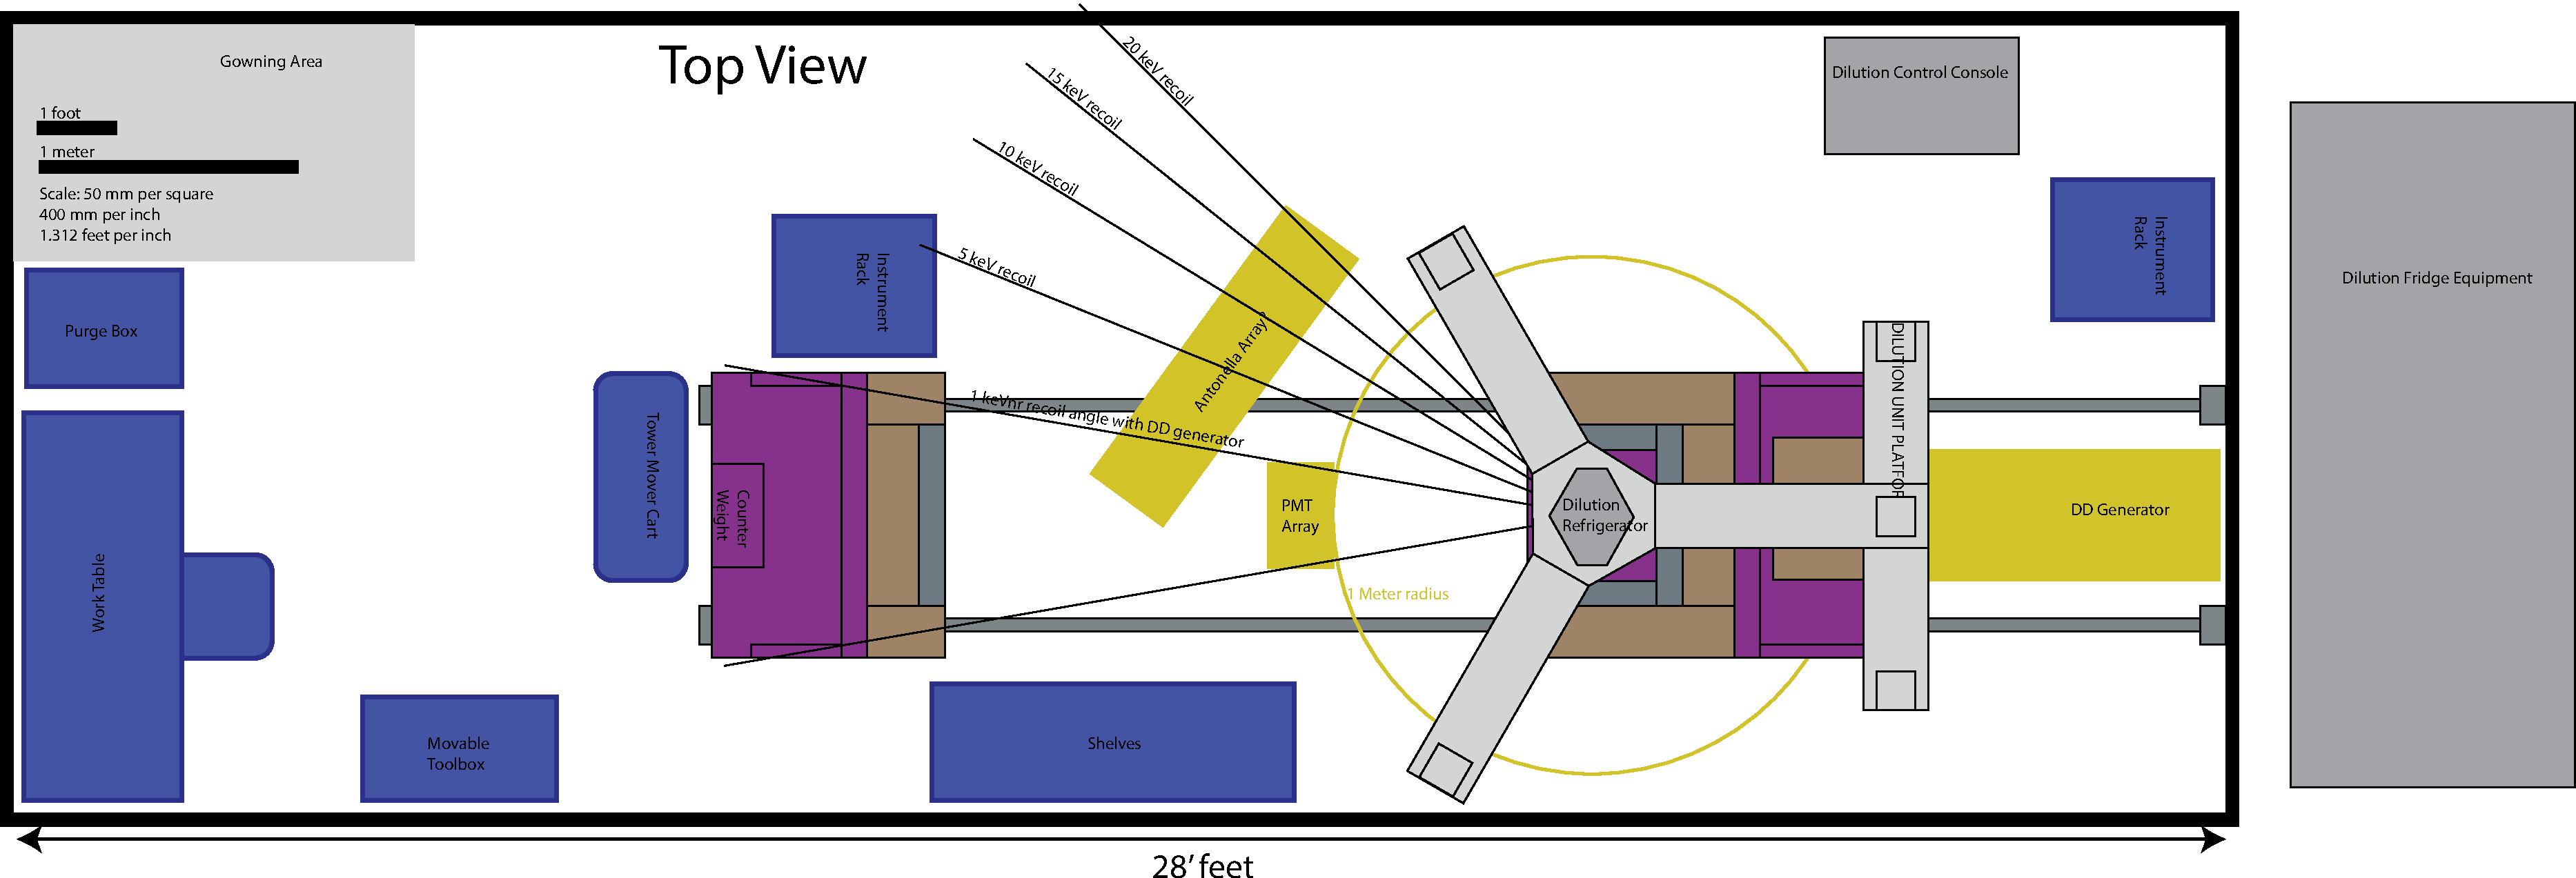
\includegraphics[width=\textwidth]{Figures/NEXUS-Layout-YieldMeas}
\caption{\nexus layout schematic. The outer box delineates the clean room to be placed 100 m underground in the \numi access tunnel. The blue boxes are support equipment, while the grey, brown, and purple structures are the passive shield, which is on rollers and half of it is moved out to the left to allow the neutron backing detectors to be placed. The D--D generator (described in Section~\ref{sec:ddcal}) is shown as a yellow box on the right, with neutrons passing through a collimating hole in the shield toward the detectors. Neutrons hit the HV detectors in the dilution refrigerator and scatter into angles as labeled depending on the recoil energy. An existing array from Fermilab will cover the wider angles between up to 20~keV, while a purpose-made fine-grain neutron detector PMT array will cover the recoil energies below 1~keV.\vspace{-2ex}}
\label{fig:nexus}
\end{figure}

\nexus is a testing facility planned for the MINOS near-detector hall at Fermilab ( 100~m underground). It will operate a dilution refrigerator surrounded by a 10~cm lead and 20~cm poly shield in a clean room environment. The rock overburden removes all muon-induced hadronic showers and lowers the muon flux to 0.5 muons/m$^2$/s. The lead shield (which includes a disk-shaped shield inside the refrigerator similar to \cute) will reduce the background to less than 100~events\perkkd. This facility is being built through a collaboration between Northwestern University and Fermilab.  A schematic of the calibration setup described in Section~\ref{sec:ddcal} is shown in Figure~\ref{fig:nexus}. The design of the clean room facility, the structural support for the dilution refrigerator, and the passive shield mechanical design are all underway. Installation of the dilution refrigerator is expected in fall of 2017, and the facility will be operational by the end of that year.


\subsection{Electronics and Shielding for \SuperCDMS Detectors}
%\comment{This probably belongs in the budget justification or somewhere else}

Much of the \scs hardware required to perform the measurements and science outlined in this proposal, such as pre-production towers and detectors, will be made available after the items are no longer needed for the \scs project. There are several exceptions, which are budgeted in this proposal and described here. To complete the measurements in this proposal at \nexus, the ability to read out two detectors is required. For \cute, a full contingent of 6 detector readout channels is needed for the science measurement. Thus we request: 

$\bullet$ Detector Control and Readout Cards (DCRCs). Two DCRC's are required to read out each HV detector, so we budget 4 for \nexus and 4 for \cute to test pre-production detectors. The HV tower will have its own DCRC's that will move to \scs with the tower.

$\bullet$ 300 K--4K wiring. The wiring to connect the DCRCs to the towers needs to be provided. Four are available for use at \cute, so we budget 8 more (we need 12 to read out the tower) and 4 for \nexus.

$\bullet$ Lead shield for \cute. The order of magnitude background reduction provided by this shield will provide sensitivity to the  \isotope[32]{Si} signal and the potential for early dark matter science. The shield for \nexus is already part of the facility.




%\clearpage

% !TEX root = NSF_SuperCDMS_SNOLAB_OPS.tex
\section{Pre-Operations and Commissioning Tasks}
\label{sec:operations}

The \SuperCDMS collaboration has had two decades of experience in operating underground dark matter experiments at Stanford and Soudan. The `lessons learned' from this experience are being applied as we develop our pre-operations, commissioning, and operations models for the \scs experiment. In this section, we discuss the main activities that will be conducted during this three-year proposal. These follow from the objectives listed in Section~\ref{sec:overview}, and are organized in a work breakdown structure as follows: 

\begin{table}[h]
\centering
\begin{tabular}{ll}
\multicolumn{2}{l}{\WBS Descriptions}\\\hline
1.1 & Calibration of Si and Ge \scs Detectors\\
1.2 & Performance Optimization of \scs Detectors \\
1.3 & Early \scs Science\\
1.4 & \scs Commissioning\\
1.5 & Education and Public Outreach\\
%\hline
\end{tabular}
\caption{Work Breakdown Structure for this proposal, based on the objectives laid out in Section~\ref{sec:overview}.}
\end{table}

The first two activities in the \WBS are measurements essential to the scientific output of the \scs experiment. The third activity provides the potential for early world-leading low-mass dark matter results, which will not only have the potential for discovery, but provide training and publications for our young scientists in the collaboration. This proposal's fourth activity is the commissioning of the \scs experiment, clearing the final hurdle for operations to begin. The final activity is the education and public outreach component of the Broader Impacts of this proposal.
The following sub-sections detail the work to be done in each of these activities.

  
%%%%%%%%%%%%%%%%%%%%%%%%%%%%%%%%
% Calibration is big so goes in its own file:
% !TEX root = NSF_SuperCDMS_SNOLAB_OPS.tex

\subsection{Calibration of Si and Ge \scs Detectors (\WBS 1.1)}
\MP{
\begin{itemize}
	\item rename to measure the nuclear recoil ionization yield at very low energies
    \item I think we should add a section on testing the electronic recoil calibration signal using LEDs
    \item we need to write this section with the understanding that 0V operation has a natural nuclear recoil ionization scale.
\end{itemize}
}

\label{sec:calibration}

A major focus of the SuperCDMS pre-operations program is to measure the nuclear recoil energy response in both Ge and Si down to 100 eV and eventually down to $\sim$30\eV.  This will match the energy thresholds we expect to achieve with the initial experiment and with upgraded detector towers.  These measurements are crucial for optimizing the operational parameters of, as well as achieving science in the next three years with the first production HV SuperTower at the Cryogenic Underground TEst (\cute) facility in \SNOLAB. Thus it is important to perform these measurements as early as possible, ideally completing them before data taking with the HV tower at \cute begins.

The signature of a WIMP-like dark matter interaction is a spectrum of low-energy nuclear recoils. \MP{WIMP DM is excluded < 10GeV ... we are looking largely for assymmetric dark matter models} The nuclear recoils produce both ionization and phonons.  The ionization yield (also know as quenching factor), which is the fraction of recoil energy that goes into the ionization, is recoil energy dependent.  A calibration of the nuclear recoil energy scale requires a measurement of the ionization yield, both its mean and its distribution, for all recoil energies of interest.

% The signature of a WIMP-like dark matter interaction is a spectrum of low-energy nuclear recoils. The observed signal in the HV detectors is a linear combination of the primary phonon and ionization signals, and is dominated by the ionization which is amplified by the Neganov-Luke effect.  This observed energy is converted to nuclear recoil energy based on understanding of the detector ionization yield (also know as quenching factor), which is the fraction of recoil energy that goes into the ionization channel.  A calibration of the nuclear recoil energy scale is hence effectively a measurement of the ionization yield. -- old text, Alan, 02/11/2016

\begin{figure}
\centering
\includegraphics[width=0.75\textwidth, trim={0 0 0 20}, clip]{Figures/Yield_Baseline_vs_Literature_SiGe}
\caption{Comparison of a simulation of the proposed ionization yield measurement compared with existing measurements of the mean ionization yield from the literature. The proposed measurement, shown following a Lindhart ionization yield model, has the potential to provide essential data on the ionization yield mean and statistical fluctuations for dark matter rate calculations in the lowest energy ranges. 
The colored scatter points correspond to the simulated ionization yield as a function of recoil energy, superimposed on the \(\pm1\sigma\) statistical uncertainty band from Eq.~\ref{eq:yielderr} (note that the blue \(\pm1\sigma\) bands only account for the statistical uncertainty due to phonon energy resolution and neutron scattering angle, whereas the actual points also include the effect of electron-hole production statistics, i.e., the Fano Factor). The gray diamonds indicate the mean value of the calculated yield from the simulation, and the vertical bars are the square root of the variance. Figure adapted from~\cite{2013APh....48....8B,1965PhRv..138.1815S,1990PhRvD..42.3211G}.
%\vspace{-3ex}
}
\label{fig:exp_vs_litt}
\end{figure}
Figure~\ref{fig:exp_vs_litt} shows current mean ionization yield measurements in germanium and silicon detectors made with a variety of detector technologies, along with the theoretical prediction from the Lindhard model~\cite{1964PhL....12..126L}. Also shown (and discussed fully in the subsequent sections) are a set of simulated yield measurements %done by the \UF group
demonstrating what would be possible with the proposed work, superimposed on the current state of knowledge of the low energy nuclear recoil yield in germanium~\cite{2013APh....48....8B} and silicon~\cite{1965PhRv..138.1815S,1990PhRvD..42.3211G,1992PhRvA..45.2104D,Chavarria:2016arXiv}. Highlighting the importance of experimental data, a recent measurement, made by the DAMIC collaboration (top panel of Figure~\ref{fig:exp_vs_litt}), indicates that the ionization yield in Si is significantly different from the theoretical predictions of Lindhard at and below 1\keV.  Projecting the deviations down to 100\eV suggests even larger discrepancies.

For SuperCDMS, the interplay of ionization yield, trigger threshold and experimental sensitivity is complex.  As the ionization signal is detected via its conversion to phonons by the Luke-Neganov effect, the total phonon signal measured includes both primary phonons from the recoil and Luke-Neganov phonons from primary ionization. In Figure~\ref{fig:SensitivityYVScanHV}, calculations for Si show how the sensitivity can vary with different ionization yield assumptions.  Furthermore, systematic bias from uncertainty in the ionization yield can be reduced and sensitivity to the lowest masses regained by operating at reduced voltage at the cost of higher background in the signal region (as demonstrated by the extreme case of 0\,V, which is used here to show the theoretical maximum effect).  Both issues demonstrate the need to measure the ionization yield of \scdmssnolab HV detectors by the time science runs at \cute begin.
\begin{figure}[htp]
\centering
\includegraphics[width=0.48\textwidth]{Figures/Sensitivity_Si_YV_Scan}
\includegraphics[width=0.48\textwidth]{Figures/Sensitivity_Ge_YV_Scan}
\caption{Left panel: Sensitivity scan of SuperCDMS SNOLAB Si HV detectors for different yield and analysis thresholds. Black is the nominal projected sensitivity, which uses the DAMIC yield function~\cite{Chavarria:2016arXiv} and extrapolates the yield curve down to 40\,eV~\cite{SuperCDMSSensitvitiy:2016arXiv}. Grey is Lindhard theory for comparison. Orange is the sensitivity projection for operation of the detector with zero voltage across the crystal. The red line shows the sensitivity from an analysis that sets the threshold at the lowest recoil energy for which data on ionization yield exists (675\,eV). The region to the left of the red line highlights the WIMP parameter space that requires new experimental data for ionization-measuring detectors. Right panel: Same as Left but for Ge HV. The black line uses Lindhard theory, orange is zero-voltage operation, and red applies an analysis threshold of 254\,eV.
%\vspace{-3ex}
}
\label{fig:SensitivityYVScanHV}
\end{figure}

\subsubsection{Measurement Strategy}

We propose to perform a precision measurement of the ionization yield in this energy range first at a neutron beam facility with small prototype detectors and subsequently using a D--D neutron generator with full-sized SuperCDMS SNOLAB detectors.  In both these setups, the energy of the incoming neutron is known and the deposited nuclear recoil energy in the detector is determined kinematically by measuring the outgoing neutron angle. By directly measuring the ionization signal in the target/detector it is then possible to perform a direct measurement of the ionization yield. 

%%%%%%%%%%\subsubsection{The Voltage-Assisted Calorimetric Ionization Detection Technique}
\SuperCDMS detectors determine the properties of a particle interaction by measuring the energy deposited in two different physical channels: the phonon and ionization channels. When an interaction takes place in the detector the total recoil energy of an interaction is initially divided among a population of prompt athermal phonons and a population of charged excitations (\textit{i.e.}, electrons and holes). A uniform electric field of a few V/\(\!cm\) causes the electrons and holes to drift to opposite surfaces where they are detected with a capacitively-coupled charge amplifier. The motion of the charged excitations in the crystal under the influence of the applied electric field creates a population of phonons known as Luke-Neganov phonons. These release to the phonon system an amount of energy equal to the work required to drift the charges through the field across the resistive crystal, i.e., $E_{Luke} = n_{eh}\,e\,V$, where $n_{eh}$ is the number of electron hole pairs made in the recoil, and $e\,V$ is the electron charge times the voltage across the crystal.  The total phonon energy $E_{ph}$ measured in the detector for a given recoil energy $E_r$ is,
\begin{equation}
\label{eq:yield}
E_{ph} = Er + E_{Luke} = E_r \left ( 1+\frac{e\,V\,Y}{\mathcal{E}_{eh}} \right )
\end{equation}
where $\mathcal{E}_{eh}$ is the average electron equivalent energy required to form an electron hole pair, $Y$ is the ionization yield

Effective ionization resolutions on the order of few eV (corresponding to individual e-h pairs) can be achieved using the technique of voltage-assisted calorimetric ionization detection which was first used by the \SuperCDMS experiment in a low-mass WIMP search using the current iZIP detectors~\cite{2014PhRvL.112d1302A,Agnese:2015nto}. By applying a high voltage (HV) across the crystal the ionization signal can be effectively amplified and measured using the phonon sensors since the energy released into the Luke-Neganov phonon population will dwarf the intrinsic recoil phonons. The detector is then being effectively operated as a phonon-based charge amplifier in which the gain of the signal is proportional to the applied voltage, and the readout channel has a fixed resolution.  The measurement uncertainty of the ionization yield, measured using Eq.~\ref{eq:yield} , the measured total phonon energy and an independent determination of the recoil energy (\textit{e.g}., from a neutron scattering angle measurement), is: 
\begin{equation}
\sigma_y= \frac{\mathcal{E}_{eh}}{e\,V}\frac{\sqrt{E_{rec}^2\sigma_{ph}^2+E_{ph}^2\sigma_{rec}^2}}{E_{rec}^2}
\label{eq:yielderr}
\end{equation}
Since the ionization yield uncertainty depends both on the phonon channel resolution and the bias voltage, a worse than expected phonon resolution can be compensated for with a higher voltage bias. %Above a bias of 500\volt , however, the uncertainty becomes dominated by the uncertainty in the recoil energy (from the event kinematics measurement), taken to be 100\eV in this calculation.

Figure~\ref{fig:exp_vs_litt} shows the result of a simulation % by the \UF group, 
with neutrons incident on a test detector with 50\eV resolution, superimposed on the current state of knowledge of the low energy nuclear recoil yield in germanium~\cite{2013APh....48....8B} and silicon~\cite{1965PhRv..138.1815S,1990PhRvD..42.3211G,1992PhRvA..45.2104D,Chavarria:2016arXiv}. This simulation shows that this experiment will have the ability to reliably identify the mean value of the ionization yield down to \(\sim 50\eV\). The horizontal spread in each population of events arises from a given neutron detector accepting a \(\pm 1\deg\) range of scattering angles.

At the improved, but still conservative, energy resolution of 10\eV (this value is twice the expected 5\eV resolution of the \SuperCDMS R\&D devices that will be used for the measurement) it becomes possible to identify the number of electron-hole pairs produced by a given recoil as shown in Figure~\ref{fig:eh_counting}. This will provide an important piece of information regarding the statistical nature of ionization production and allow us to perform a direct measurement of the Fano factor down to the lowest recoil energies.

\MP{include quantization plot from Stanford.  Switch plots to show quantized sensitivities}

\begin{figure}[t]
\centering
\includegraphics[width=\textwidth]{Figures/Phtot-Hist-Neutron-beam-HiRes-G4}
\caption{
Demonstration of the ability to identify the number of discrete electron-hole pairs (indicated by the dashed vertical lines) created by a low energy nuclear recoil. The combination of high bias voltage and excellent energy resolution allows for the measurement of the Fano factor even with limited statistics.
%The figure is based on simulations performed by the \UF group.
%\vspace{-2ex}
}
\label{fig:eh_counting}
\end{figure}

\subsubsection{Yield Calibration with a Neutron Beam at TUNL (\WBS 1.1.1)}
\label{sec:tunl}

The Triangle Universities Nuclear Lab (\tunl) data taking campaign will occur in the first year of this grant (see schedule in Figure~\ref{fig:ops-schedule}). \tunl operates a facility capable of delivering a mono-energetic neutron beam with energies in the range of 30\keV to a few\MeV~\cite{TUNL:website,Theprecisionquench:2014tw}. A tandem Van de Graaff is used to accelerate protons and collide them with a \isotope[7]{Li} target. The resulting \isotope[7]{Li}(p,n)\isotope[7]{Be} reaction produces a neutron that is primarily collinear with the proton beam. At a proton threshold energy of 1.88\MeV the reaction produces neutrons with 29.7\keV kinetic energy which are kinematically constrained to be in the forward direction. Increasing the proton energy allows for the production of neutrons with a range of kinetic energies and directions, however by selecting a particular direction (e.g. collinear with the proton beam) a unique neutron energy is obtained~\cite{1999NIMPB.152....1L}.

The neutron beam passes through a 2 foot high-density polyethylene (HDPE) block which collimates the beam and absorbs unwanted reaction products (such a \(\gamma\)-rays) and is directed to the target location. Backing detectors  (5cm inch diameter plastic scintillator, with sensitivity to neutrons down to 6\keV) surround the interaction site and detect the scattered neutron providing knowledge of the scattering angle and timing of the event, and can be positioned around the interaction point as needed. The TUNL facility currently has 32 such detectors and is in the process of deploying 200 more to provide a solid angular coverage of almost \(1\pi\) steradian. The additional neutron detectors are expected to become available in January of 2017. One of the most useful features of the facility is its ability of providing a pulsed beam, which in conjunction with the backing detectors' timing resolution of \(< 4\,\)ns allows for an excellent rejection of events due to pileup, multiple scatter or radioactive backgrounds, and also provides a secondary measure of the neutron energy through its time-of-flight.

The details of the backing detector configuration will be investigated and optimized in the early stages of the proposed work plan in order to obtain an experimental setup that allows for making the measurement at the the desired level of accuracy in a minimum amount of beam time.

%%%%%%%%%%\subsubsection{Calibration at a Neutron Beam Facility}
%Calibration at a neutron beam facility, such as TUNL~\cite{TUNL:website}, is attractive because the beam energy can be tuned as low as $\sim$30\keV and an extensive secondary neutron detector array is available for use~\cite{Theprecisionquench:2014tw}. 
The Northwestern \SuperCDMS group owns an Adiabatic Demagnetization Refrigerator (ADR) that can be transported to TUNL to perform such a measurement.  The ADR can cool small, special-purpose Ge and Si HV detectors, each with mass of a few grams. Detectors of this size are produced as part of the \SuperCDMS R\&D program and are available for these measurements. Two such detectors (one made of Si, one of Ge) will be installed in the ADR so the \tunl measurements can be done without warming up or opening the cryostat.

The kinematics at a neutron beam result in an excellent recoil energy resolution: for a \(1\deg\) uncertainty in the direction of the scattered neutron, the reconstructed energy resolution is on the order of 4\eV for a 100\eV recoil. This value is close the the expected 5\eV resolution of the \SuperCDMS phonon sensors, and as seen in equation~\ref{eq:yielderr}, is optimal for achieving excellent ionization yield resolution. The neutron beam measurements will be used to obtain the highest resolution ionization yield measurements at the lowest energies allowing us to study in detail the physics and statistics of electron-hole pair production via nuclear recoils at their creation threshold.


\subsubsection{The TUNL Experimental Campaign}

The simulation in Figure~\ref{fig:exp_vs_litt} assumed \(10^3\) events for each recoil energy. We investigated a feasable set of operational parameters necessary for obtaining such statistics in the actual data while minimizing the amount of multiple scatter, pileup and background events in the data. The two driving variables are the detector response time, and the interaction probability of a neutron with the detector. 

Based on a conservative detector recovery time of \(\tau=1ms\) we wish to keep the interaction rate in the detector below 100~Hz to minimize pulse pileup. The mean free path of 30\keV neutrons in silicon (germanium) is \(\sim 2cm\) (\(\sim 2.3cm\)), which gives a 18\% (16\%) probability for a single neutron to interact in the 4mm thick test detector. This can lead to a large number of simultaneous interactions in the detector from a single beam pulse contaminating the data. This effect can be mitigated by decreasing the average number of neutrons per beam bunch. A mean number of neutrons per bunch of \(n_{mean}=0.4\) results in less than 3\% contamination from simultaneous interactions. The combination of \(n_{mean}=0.4\) and a bunch frequency of \(\frac{1}{600\mu s}\) results in a net detector interaction rate of 100~Hz. Such an operating mode is well within the capabilities of the facility and given the $< 4$~ns timing resolution of the backing detectors there will be no difficulties distinguishing which beam bunch produced a particular interaction~\cite{barbeau:2014}. Assuming that each backing detector covers an angle of \(\left( 1\deg\right)^2\), that they are positioned in groups of 10 at each of 20 angles, and that the net neutron interaction rate in the detector is 100~Hz, we can estimate the total active beam time required to obtain the necessary statistics to be around 12 hours. The data for the different recoil energies is collected simultaneously by the grid of \(>200\) backing detectors at 20 specific scattering angles. Assuming a net efficiency of five to six hours of beam time per calendar day, it is reasonable to expect that a data acquisition period of a few days is sufficient for a particular measurement. Data will be taken for both a prototype Si and Ge detector, at multiple bias voltages and operating conditions (such as crystal temperature) during a three week running window. An additional week before and after the data acquisition campaign for assembly/disassembly and verifying the operation of the detector at the TUNL facility will also be required.

\subsubsection{Data Contamination}
\begin{figure}[tb]
\centering
\includegraphics[width=0.45\hsize]{Figures/single_multiple_scatters_geant}
\includegraphics[width=0.45\hsize]{Figures/Delta_t_histograms}
\caption{Left panel: %Distribution of 
Energy deposited in the detector as a function of neutron scattering angle. The orange band band represents events in which the neutron scattered only once within the detector without interacting with the surrounding material. Events which multiply scatter within the detector are shown in blue, and events which interact with the Al or Cu surrounding the detector are shown in green and red respectively. Right panel: Histogram of the event delay times, i.e. the time between the arrival of a beam bunch and the detection of a neutron in the backing detectors. The delay was defined such that \(\Delta t=0\) for a non-scattered neutron, and the backing detectors' timing resolution is \(< 4\,\)ns.
\vspace{-3ex}
}
\label{fig:geant}
\end{figure}

Environmental radiation background and neutron interactions with the material surrounding the detectors have the potential to contaminate the data. A proper understanding of these interactions requires a detailed Monte-Carlo simulation. The results from a basic \geant simulation done by our U. Florida collaborators and shown in Figure~\ref{fig:geant} are still quite informative. They simulated the interactions of a neutron beam with a detector surrounded by a 1mm thick copper housing, contained in a 1cm thick aluminum cylindrical shell (which represents the cryostats vacuum jacket). The figure's left panel shows the distribution of energy deposited in the detector as a function of neutron scattering angle. The thick orange band represents events in which the neutron scattered only once within the detector without interacting with the surrounding material.  Multiple scatters within a detector, as well as events in which the neutron interacts with the surrounding material are also shown. The right panel shows the delay time distribution (the time between the arrival of a beam bunch and the detection of a neutron in the backing detectors). It can be seen that a time based acceptance cut can remove a large portion of multiply scattered events and interactions in the surrounding material. It is worth noting however, that even without applying any selection criteria, the simulation shows that contamination from such events is less than 5\% for all recoil energies \(< 1\keV\).



\subsubsection{D-D Generator Measurements at NEXUS (\WBS 1.1.2)}
\label{sec:ddcal}

\MP{What about testing the concept of measuring nuclear recoil ionization yields with Cf by measuring 0V, 50V, 100V. This would give us the possibility of using Cf for insitu calibration of all detectors in SNOLAB (or at NEXUS) extremely easily}

There are several challenges associated with calibrating large cryogenic solid-state detectors in a fixed neutron beam.  These massive detectors require a dilution refrigerator to operate at millikelvin temperatures, and such refrigerators are not portable.  Adiabatic Demagnetization Refrigerators, although portable, lack the cooling capacity to effectively operate these detectors. Furthermore, underground calibrations are critical for large cryogenic detectors. When operated on the surface, the time between events from cosmic radiation can be less than the recovery time required for the phonon sensors to return to equilibrium. \MP{this just isn't true. We have a compton background of 40Hz (25ms) and a falltime which is <100us ... we have 250 falltimes on average between comptons. The bigger problem is muons [perhaps what you were referring to] ... muons occur @1Hz and have a 200ms thermal falltime.  We find that with a muon cut with 50\% passage, we get rid of this to the point that it's subdominant to other noise sources ... it's definitely a penalty (50\% livetime) ... but it's not a true deal breaker ... remember that the livetime of our old DAQ was only 15\%. We still take more good data now with the muon cut then we ever took with the old DAQ at UCB)}.

The portability of a D--D generator allows for neutron calibration at underground locations, such as \nexus, described in Section~\ref{sec:nexus}. 

%MOVED to NEXUS section
%\begin{figure}[t]
%\centering
%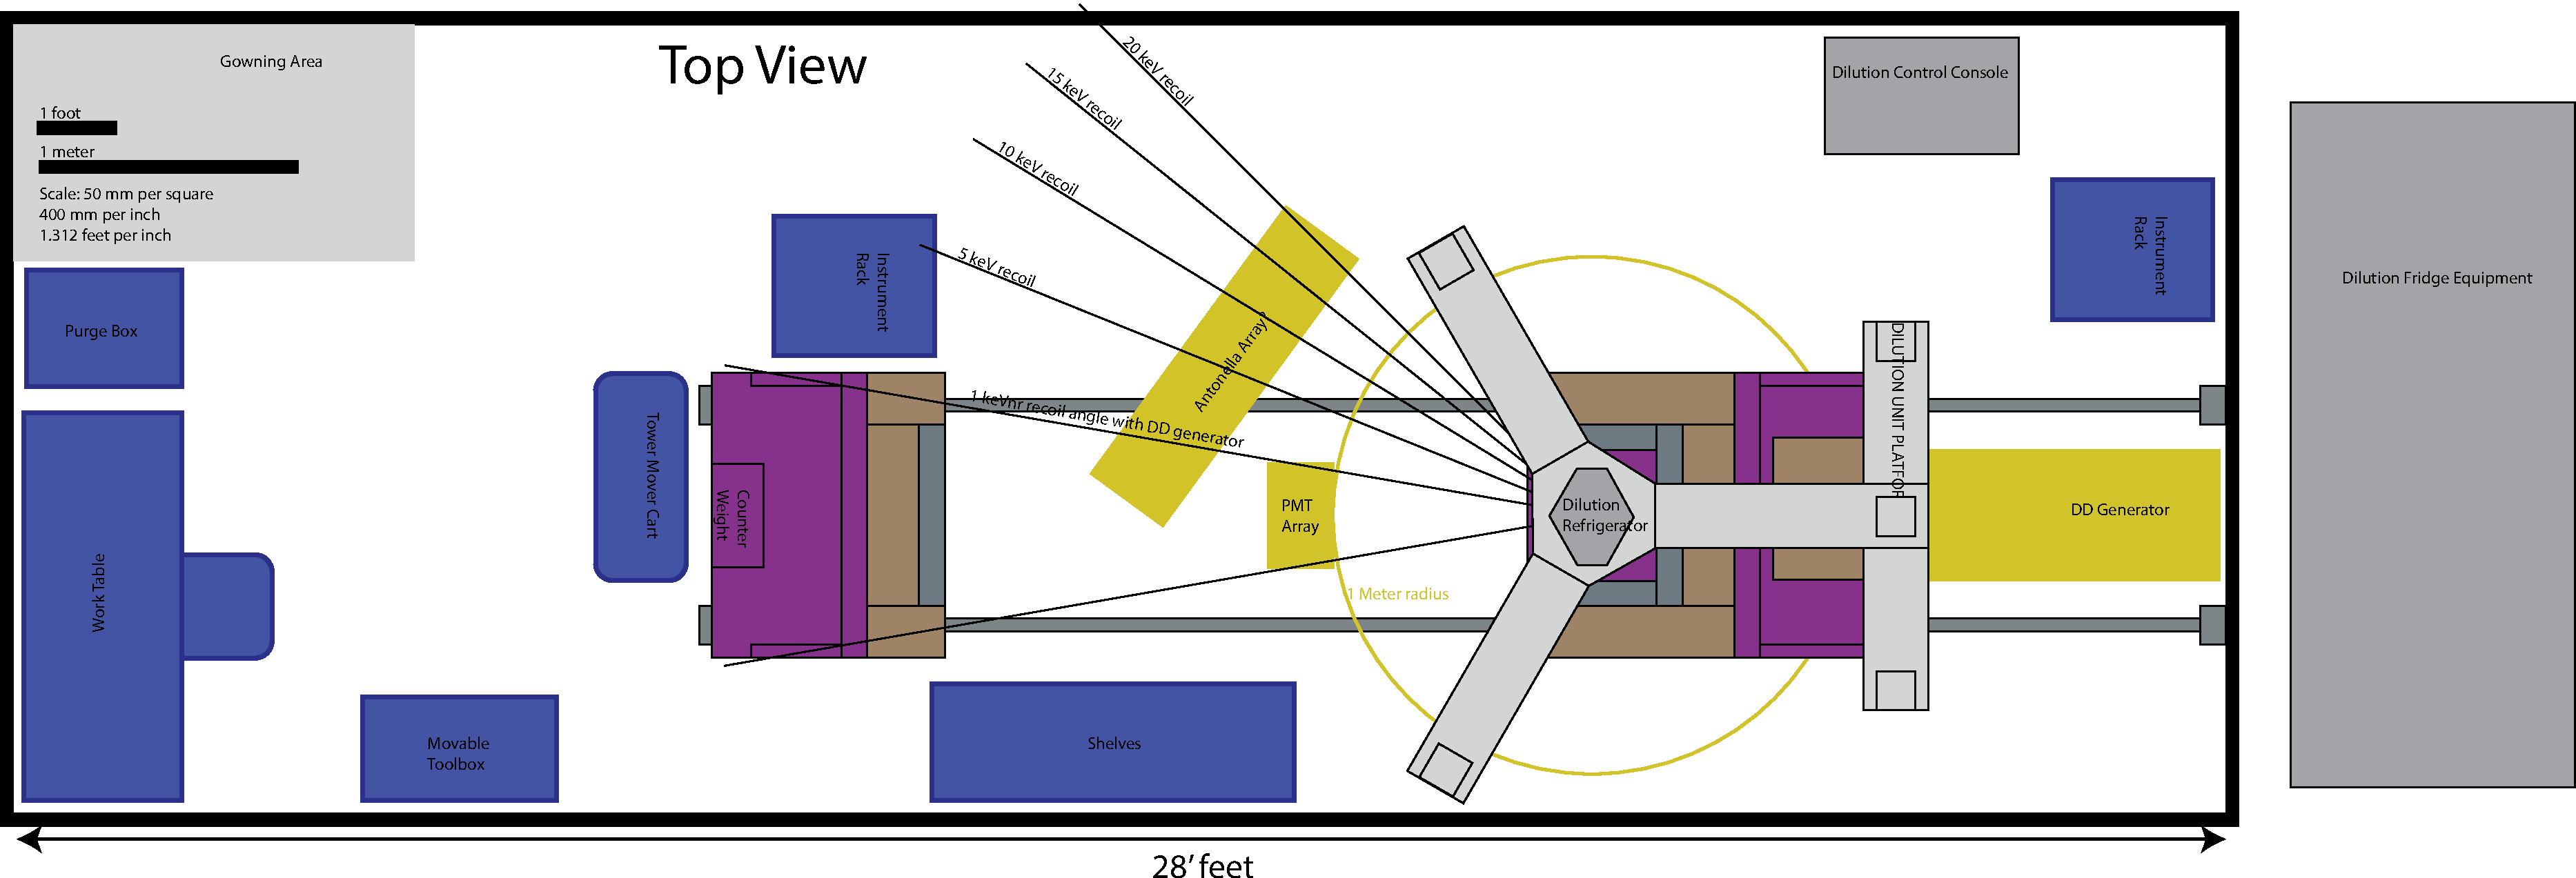
\includegraphics[width=\textwidth]{Figures/NEXUS-Layout-YieldMeas}
%\caption{\nexus layout schematic. The outer box delineates the clean room to be placed 100 m underground in the \numi access tunnel. The blue boxes are support equipment, while the grey, brown, and purple structures are the passive shield, which is on rollers and half of it is moved out to the left to allow the neutron backing detectors to be placed. The D--D generator is shown as a yellow box on the right, with neutrons passing through a collimating hole in the shield toward the detectors. Neutrons hit the HV detectors in the dilution refrigerator and scatter into angles as labeled depending on the recoil energy. An existing array from Fermilab will cover the wider angles between up to 20~keV, while a purpose-made fine-grain neutron detector PMT array will cover the recoil energies below 1~keV.\vspace{-2ex}}
%\label{fig:nexus}
%\end{figure}


Calibration with a D-D generator requires borated poly shielding to collimate the D-D neutrons into a beam and a moderate amount of lead shielding to block the capture gammas. Additionally, secondary neutron detectors are needed to measure the scattered neutrons at a given angle.  The ANTONELLA collaboration has a neutron detector array, that was created exactly for this purpose and is currently available for use.  This array covers relatively large angles of scatter ($>$10$^\circ$).  With this array, we can measure nuclear recoils down to a few keV with the D-D beam energies.  Measurement down to 100 eV requires fabrication of a finer-grained neutron array. Design of such an array, with the reuse of 1.3 cm Hamamatsu photomultiplier tubes salvaged from the SELEX experiment, will be pursued by the U. Florida and Fermilab groups. The setup is schematically shown in Figure~\ref{fig:nexus}.

\MP{Has this array been procured?  If not then you are just doing nuclear recoil ionization yield measurements @ a few keV}

In \SuperCDMS detectors, there are energy-scale effects that are degenerate with measurement of the ionization yield and can vary with detector parameters such as the strength of the electric field, fabrication of the phonon sensors, and even the impurity levels in a given crystal.  To understand these systematic effects, it is important to perform the calibration on detectors that will have the same electric field and style of phonon sensor.  Furthermore, it is highly desirable to perform measurements on several different detectors of the same type, operated at several bias voltages.  \MP{explain} 

The primary challenge of the D--D calibration is the relatively high energy (2.5\MeV) of the neutrons compared to the recoil energies of interest (100\eV). For a \(1\deg\) uncertainty in the direction of the scattered neutron the reconstructed energy resolution of a 100\eV recoil becomes \(\sim 30\eV\). This uncertainty becomes the limiting factor in the measured yield resolution. One way to compensate for this effect is to use a fine-grained neutron array to determine the neutrons' very small scattering angles. An angular resolution of \(\sim0.125\deg\) is needed to achieve the same recoil energy resolution as with the 30\keV\ \tunl neutron beam. The resulting scattering rates per secondary neutron channel will be approximately 60 times lower compared to the rates at a neutron beam facility. The lower detection rates, in turn, lead to longer data acquisition times and an increased sensitivity to environmental backgrounds. Studies will optimize the tradeoff between recoil energy resolution and the impact of data contamination sources such as background interactions in the neutron array and multiple scattering of the D--D neutrons both within the \SuperCDMS detectors and the surrounding material of the dilution refrigerator. 

The neutron beam and D--D setups will experience different experimental systematic effects.  By taking data with the small calibration detectors at the D--D generator setup, we can correlate the neutron beam and D--D systematics, and use this understanding to extrapolate the high-resolution beam data to the kg-size detectors.  Thus a cross-calibration would provide robustness to our understanding of the ionization yield and provide additional higher-resolution data points in the energy region where currently no data exists. The data with the small HV detectors at \nexus will be taken in the latter part of Year 1 of this grant. Year 2 of the grant will be devoted to pre-production \scs detector calibration (see schedule in Figure~\ref{fig:ops-schedule}).
%We will also investigate the possibility of operating at the same angular resolution as that of the TUNL facility (\(1\deg\)), and using the information from Monte-Carlo simulations and the TUNL measurements to extract high resolution ionization yield information at low energies from the D--D measurement.

The D--D calibration setup will enable a program of measurements that can explore the calibration differences that arise with different operating conditions and detector designs.  This will lead to a full understanding of the systematic uncertainties associated with ionization production in \SuperCDMS detectors. 

%Summary
In summary, the \tunl \& \nexus campaigns enable a program of measurements that can obtain high-resolution physics measurements of the ionization yield of Si and Ge at recoil energies down to 100~eV and below, explore and correct for systematics in the measurements, and perform direct measurements of the ionization yield of \scs detectors.  This will enable a full understanding of the systematic uncertainties and provide essential inputs for the dark matter science analysis of \scs data.


%%%%%%%%%%%%%%%%%%%%%%%%%%%%%%%%%
\subsection{Detector Performance Characterization and Background Studies (\WBS 1.2)}

\MP{
\begin{itemize}
	\item Nuclear Recoil Ionization Yield Measurement
    \item testing optical photon calibration techniques
    \item Charge Leakage Studies
    	\begin{itemize}
        	\item optimize pre-bias voltage
            \item optimize LED/blackbody frequency for A+,D- 
            \item optimize bias voltage
        \end{itemize}
    \item Electronic Recoil / Nuclear Recoil Discrimination
    	\begin{itemize}
        	\item Quantization / Statistical subtraction in HV 
            \item Standard ER/NR in iZIP
        \end{itemize}
    \item Fiducialization Metrics 
    \item (@ Berkeley) noise studies with small TES chips
\end{itemize}
}

The \MP{Nuclear Recoil / Electron Recoil?} discrimination power and general behavior of \scs detectors under low-background conditions cannot be tested in regular detector test facilities due to the high rate of cosmic ray induced interactions in the detectors. A large focus of this proposal is to make such measurements at \nexus and \cute. 

\MP{why not discuss charge leakage optimization specifically?}

\subsubsection{Detector Characterization with NEXUS}

Although the nuclear recoil energy calibration (described in detail in section~\ref{sec:calibration}) will be the main focus at \nexus, having pre-production detectors at the site will also allow early detector characterization. The  ability to kinematically reconstruct nuclear recoil energies, as well as the flexiblity to place and remove gamma sources, will faciliate studies that impact the analysis and interpretation of the \scs data. 

\MP{these are all really important ... they should have similar size at the nuclear recoil ionization yield work if possible}
These include position dependence and specific detector Monte-Carlo tuning studies (see Section~\ref{sec:dmc}), voltage bias scan studies, and other studies such as measuring single electron-hole pair production using optical fibers. 
The goal of the optical fiber studies will be to directly measure the separation between integer numbers of electron hole pairs near the threshold of HV detectors as a means to confirm the electron recoil energy scale near threshold.  The optical fiber setup also allows for studies of charge collection, which could inform operating procedures for the main experiment. These measurements will take place during Year 2 of this proposal, at the end of each detector's calibration measurement. 

\subsubsection{Background Studies and Precommissioning with CUTE}
\label{sec:CUTE}

A primary goal in the design of the \cute facility is to test the capability of the \SuperCDMS HV and iZIP detectors to distinguish surface from bulk events (fiducialization). The discrimination power between electron and nuclear recoils of the \SuperCDMS iZIP detectors can also be studied in detail. Additionally, functionality and early commissioning checks of a tower can be performed before it is deployed within the main \SuperCDMS cryostat.  Functionality checks would verify that electrical and thermal connections in the tower are functioning properly after shipment to \SNOLAB. Early commissioning checks include optimization of voltage bias and neutralization studies.  These tests are best performed in a low-background installation such as \cute because breakdown voltage and optimal neutralization conditions have previously been found to  correlate with event rate.

Recent measurements of detectors used for \SuperCDMS \Soudan have shown that the noise in the signal region increases linearly with the applied bias voltage. Such behavior would limit the sensitivity of the new \SuperCDMS HV detectors that are designed for operation with up to 100~V bias. The origin of this excess noise is not yet fully understood. Possible explanations include infrared leakage and injection of charges through the contacts. Low-angle Compton scattering has been identified as alternative explanation; this would also explain why the observed noise level appears to be the same in different test facilities with no, or only moderate, shielding.

\MP{where did this theory come from? ... why would there be a huge number (1e5Hz) of single e/h pair comptons?}

We will test this hypothesis and understand the behavior of the new \SuperCDMS HV detectors in \cute's low background environment.

As shown in the schedule (Figure~\ref{fig:ops-schedule}) we expect to install in \cute one of the two pre-production towers at the beginning of calendar 2018 after the tests planned by the \scs Project are finished. This tower is intended to have two pre-production HV detectors and one pre-production iZIP.

After 2 months of commissioning and basic checks of performance, we plan a 9-month testing program to study:
\begin{compactitem}
\item  Fiducialization and surface rejection in HV detectors.
\item  Nuclear recoil discrimination of iZIP detectors.   
\end{compactitem}

\subsubsection{Detector Monte-Carlo Validation}
\label{sec:dmc}

The \SuperCDMS collaboration is currently in the process of building a \geant based detector Monte-Carlo that incorporates low-temperature ionization and phonon physical processes governing the behavior of electrons, holes, and phonons in the \SuperCDMS detectors. The physical processes being added to \geant include:
\begin{compactitem}
\item A microscopic model of inter-valley scattering for charge charge carriers in the crystal.
\item Luke-Neganov phonon emission based on the charge carrier mean free path in a varying electric field.
\item A continuous process of phonon impurity scattering.
\item The creation and tracking of quasiparticles in the the Al superconducting films that at part of the phonon sensors.
\item Differential equation based models of the FET (ionization sensor readout) and TES (phonon sensor readout) responses.
\end{compactitem}

Data from the \tunl and \nexus campaigns will consist of a set of nuclear recoil events with well defined kinematics.  Additionally, the data obtained  from the precommissioning calibration at \cute will provide a large set of events from gamma and neutron calibration sources taken in a low background environment. 
These data sets will provide a comprehensive collection of events for comparing against Monte-Carlo simulations. The data will be made available to members of the \SuperCDMS collaboration who are working on detector Monte-Carlo and simulation activities and are validating the performance of the detector Monte-Carlo, and refining it in preparation for the \scs experiment. %Funding for such work, however, is not part of this proposal.

%%%%%%%%%%%%%%%%%%%%%%%%%%%
\subsection{Early \scs Science (\WBS 1.3)}

One of the attractive features of the plan we propose for \cute is that it not only will give us the opportunity to exercise our detectors in a low background environment but that it might allow us to get early science results.
While the characterization of the pre-production detectors described in \ref{sec:cute} is taking place in calendar 2018, the \scs Project is scheduled to complete the first production HV tower.  We are proposing to install this first tower in \cute at the beginning of 2019 (Figure~\ref{fig:ops-schedule}). This tower would have 6 HV detectors, with a mix of Germanium and Silicon.  
Our first goals will be to:
\begin{compactitem}
\item  Assess the performance of these detectors in a realistic environment (voltage limits, leakage current, background level)
\item  Develop biasing schemes for the HV detectors
\item  Learn what small detector or cold hardware modifications we could include in the second HV tower, being produced in 2019, to optimize its performance
\item Exercise our data acquisition system, optimize our reconstruction software and begin to develop the algorithms for science analysis
\end{compactitem}

Achievement of these goals would be very beneficial to the subsequent commissioning of the \scs experiment. If all goes well, there is a reasonable prospect for doing early science with the HV tower in \cute, which is the main justification for  installing the additional lead shield that we propose to acquire in this award. Current simulations indicate that we could decrease the gamma background from 30 events/kg/keV/day to about 2 events/kg/keV/day with the additional lead shielding. In that case, a six-month HV tower run at \cute, with a baseline phonon resolution of 10 eV r.m.s. and 100 V bias (\scs goal) and the projected $^3$H and $^{32}$Si levels for \scs, might give a spin independent sensitivity as much as 4 orders of magnitude better than the current best limit \cite{2012EPJC...72.1971A} at a dark matter mass of 2 GeV/c$^2$ with Germanium, roughly a year before our first results from the \scs experiment will become available. 
%The improvement could be as large as a factor 2000 at 1 GeV/c$^2$  with our Silicon detectors. This would be only 20 times worse than the first result that we should obtain at \scs for Germanium with optimal interval method \cite{Yellin:2002xd} and about a factor six times worse for Silicon, if the $^32$Si is at the level indicated by DAMIC for a bulk contamination.  

Of course, \scs will then go on to produce much better sensitivity and reach to even lower mass. The two iZIP towers that will be included in the first \scs payload will provide an independent measurement of the background, which should yield an additional factor of 5 in sensitivity over the no-background-subtraction projections in~\cite{SuperCDMSSensitvitiy:2016arXiv}. Moreover, the second HV tower planned for the first \scs payload will have benefited from the experience of the first tower at \cute and is likely to perform better. In the long run, the \scs set up is designed to allow us to reach the neutrino floor, well beyond what will ever be possible at \cute.
Still, the potential sensitivity of a run of the first HV tower at \cute is an exciting science opportunity and will provide theses for our graduate students and interesting publications to further the career of our younger scientists.

%%%%%%%%%%%%%%%%%%%%%%%%%%%
\subsection{\scs Commissioning (\WBS 1.4) }

The \scs Project will include acceptance tests of all parts of the experimental apparatus at the surface. The Project objective is to complete the  installation of all equipment underground at \SNOLAB, although the Project threshold does not require this. \scs Operations will pick up any remaining installation tasks, then commission the experiment and transition to operations. We expect this period to occupy approximately the last six months of this proposal's performance period.

The commissioning period will be a mix of installation and testing of subsystems, followed by system testing and data runs that exercise the full experiment. System experts will be responsible for testing and documenting their equipment, with work coordinated by an on-site commissioning czar. The initial focus will be on the cryogenics system, since a successful cool down of the experiment to base temperature is required before detector tower commissioning is possible. In parallel, the readout electronics, data acquisition/trigger and software chain can be exercised. Once base temperature has been established, the focus will shift to commissioning the detector towers, using gamma and neutron sources for calibration. iZIP and HV detector towers will be studied in parallel, and the electronic noise and vibration environment will be characterized. 

As system commissioning matures, the operations manager and operations team will begin to take overnight data runs and examine the data along with the commissioning czar and system experts, to find any subtle problems. The data quality monitoring system will be commissioned, as well as the data pipeline and processing systems. Towards the end of commissioning period, we will be running most of the time, with scheduled down times to fix any problems that have been identified. During this period, the operations documentation needs to be finalized.  

NSF-funded scientists will play key roles in commissioning, with a special focus on areas covered by this proposal, especially detector performance and  calibration.  Data from pre-operations studies will be extremely useful in making sure that commissioning is smooth and that the experiment can begin taking dark matter search data as quickly as possible.

%\clearpage

% !TEX root = NSF_SuperCDMS_SNOLAB_OPS.tex

\section{Schedule}
\label{sec:schedule}

Figure~\ref{fig:ops-schedule} gives a broad view of the activities of the \SuperCDMS collaboration  centered on the \scs experiment, including the DOE/NSF G2 Project, the pre-operations and commissioning period covered by this proposal, the actual operation of \scs (also detailed in the Experimental Operations Plan), and the R\&D program that will naturally lead to upgrades for \scs that allow it to probe the low-mass dark matter region down to the neutrino floor.

% The detailed schedule for this proposal is shown in Figure~\ref{fig:ops-schedule}. 

% \begin{figure}[htb]
% \begin{center}
% \includegraphics[width=\textwidth]{Figures/supercdms_operations_schedule_nsf_ops.pdf}
% \end{center}
% \caption{\footnotesize First draft of an interleaved schedule for the \scs Project, Operations and R$\&$D and Upgrades.}
% \label{fig:proj-schedule}
% \end{figure}

\begin{figure}[htb]
\begin{center}
  \includegraphics[width=\textwidth]{Figures/OpsSched-rac.pdf}
\end{center}
\caption{Schedule for the \scs Experiment.}
\label{fig:ops-schedule}
\end{figure}

\noindent\textbf{Year 1: 7/2018--6/2019}\\
During the first year the focus will be on calibration of the small HV test detectors from Stanford University with the Northwestern ADR at \tunl. These detectors will then be taken to \nexus, to perform cross-calibration measurements in preparation for the large detector calibrations. The first pre-production detectors arrive at \cute in January 2018, and the performance  and background measurement campaign begins soon after. 

\noindent\textbf{Year 2: 7/2019--6/2020}\\
The second year is dominated by runs of pre-production detectors at \nexus for calibration and at \cute for performance testing and background measurements. The first production \scs HV tower arrives at \cute in 12/2018, with testing commencing in 1/2019. Performance and run optimization of all six detectors of the HV tower will continue until 6/2020.

 \noindent\textbf{Year 3: 7/2020--6/2021}\\
There is no activity planned for \nexus on this grant in the third year. At \cute, the \scs HV tower science run will be taking data until 11/2019, when the tower will be taken out of \cute to prepare it for installation in the \scs experiment. Commissioning activities for \scs will be the main focus of this grant in the last six months of the award, along with the collaboration-wide effort in analysis and publication of all the data products from this work.

%\clearpage

% !TEX root = NSF_SuperCDMS_SNOLAB_OPS.tex
\section{Management}
\label{sec:management}
% RASCI chart?
% SWOT analysis?
% https://www.wrike.com/workspace.htm?acc=2707966#path=folder&id=335439022&a=2707966&c=timeline3&so=10&bso=10&sd=0&st=nt-1
% https://prod.teamgantt.com/gantt/schedule/?ids=1562286#&ids=1562286&user=&custom=&company=&hide_completed=false&date_filter=&color_filter=
% https://instagantt.com/r#

The management team of this NSF collaborative proposal will be chaired by the Northwestern PI and consist of all the PI's and Co-PI's of the proposal.  They will interact with the \nexus, \cute, and \SNOLAB facility managers to coordinate all the activities delineated in this proposal, as well as with the \SuperCDMS Collaboration for science analyses and training of students and postdocs.

The work funded by this proposal is part of the full set of \scs operations and commissioning activities, some of which are outside the scope of this proposal and are funded by DOE or Canadian funds. The management team for this proposal will be in close coordination with all parties involved in the \scs Project and Operations, as well as R\&D, and other \SuperCDMS Collaboration activities. These multi-agency collaboration-wide activities will be coordinated by a team consisting of the SuperCDMS SNOLAB Project and Operations Managers, the SuperCDMS Spokesperson, and the NSF Operations PI. This team will meet regularly to coordinate activities. 

The early operations phase of the \scs experiment covered by this proposal is when it is both necessary and appropriate to ramp up the operations management and support functions for \scs, which should all be in place for the commissioning phase of the experiment in order to ensure a smooth transition to the operations phase as quickly as possible.
%We are including a 10\% risk management overhead for the commissioning part of the proposal, as the success of commissioning will directly affect the much larger \scs Experiment. 

The detailed planning for commissioning of \scs will be led by a scientist identified to be the \scs Commissioner, with this role naturally evolving into that of a Run Coordinator during the operations phase. Details of the operations phase functions and management (which are outside the scope and period of performance of this project) are given in the \scs Experimental Operations Plan.
  
%
%Project Management and Operations Management will meet regularly to coordinate activities. Although operations activities are not part of the Project scope, some coordinated sharing of equipment and personnel can be expected. During the pre-operations phase, the Project will have the final decision on all equipment built with project funding and will have priority on use of technical personnel. The Project and Operations team will work together with the Collaboration management on sharing the effort of scientific personnel.   

\subsection{Facilities Management}
Since much of the work in this proposal occurs in dedicated underground facilities, we outline here the management of these facilities and their relationship to this grant's management.

\subsubsection{NEXUS}
The \nexus facility will receive primary management oversight from the Northwestern PI. In addition, \SuperCDMS collaborators at Fermilab will provide support to interface with Fermilab as needed. A fraction of an FTE will be provided by this grant for an operations manager, to oversee the activities delineated in this proposal. 

\subsubsection{CUTE}

The \cute facility will receive primary management oversight from our collaborators at Queen's University. This grant's management team will coordinate with Queen's to oversee the \cute activities delineated in this proposal.

\subsubsection{SNOLAB}

As mentioned above, the commissioning of \scs is an activity coordinated at the collaboration level. The PI of this grant will be part of the Operations Management team and will work closely with the \scs Operations Manager to coordinate and integrate the NSF-sponsored commissioning work with the overall multi-agency commissioning effort. \SNOLAB conducts a Gateway review process for projects which includes pre-operations activities, operation of the experiment, and decommissioning. For Gateway 1 and 2, the Project Director is the primary contact for review of the design and fabrication of the \scs experiment. For Gateway 3 and 4, the Operations Manager is the primary contact for review of the experiment pre-operations and operations. The Collaboration Canadian PI is involved in all interfaces between \scs project and operations and \SNOLAB management.  This grant's PI will be in close coordination with the Project Director, the Operations Manager and the Canadian PI to oversee the commissioning activities supported by this proposal.

%\clearpage

% !TEX root = NSF_SuperCDMS_SNOLAB_OPS.tex
\section{Broader Impacts}
\label{sec:broad}

The fundamental goal of the proposed work is to make data easily accessible to individuals who want to answer science questions.

%This work is immediately useful to the PI's own collaboration and - if the work is successful - useful to practicing scientists who can more-easily extract information from their datasets.

The immediate target audience for this work are active scientists, early-career researchers, and undergraduate students who are participating in research that require access of data for which there is not a good program.  This software will reduce the time the community spends on software development.  

The intent of this work is also to make access to science more equitable.  
\begin{itemize}
    \item High quality documentation makes the software easier to use for scientists with all levels of computing backgrounds
    \item Contribution documentation and tutorials increase the pool of contributors
    \item An online resource that provides findable materials on basic concepts in scientific computing makes it possible for novices to use the software
\end{itemize}

These aspects of the work increase science access in every case to individuals without existing background in computing.  They also increase science access to access to limited lab or institutional resources: 

\begin{itemize}
    \item Researches at undergraduate-only institutions often struggle to train undergraduates to work in a custom computing environment unless they have funding for a postdoc
    \item Lab staff and a pool of experienced graduate students and postdocs can help with undergraduate and graduate student training, but these resources are not available at many institutions.
    \item Even at institutions with significant resources for training and mentorship, access to these reasons is not always equitable.  
\end{itemize}

Large numbers of students are getting their education at community colleges and four year institutions.  Complex, poorly-documented software infrastructure that gates scientific work is an unnecessary burden on faculty at these institutions and poses a higher barrier to students because they are less likely to have access to informal computing support structure than their peers at research institutions.

The proposed work will create the kernel of an ecosystem that is usable, well-documented for both novices and experts, and enjoys the support of a community that is accessible online.  The PI believes that this infrastructure is a minimum requirement for equitable access to science analysis.



\textbf{Undergraduate Education}
Direct detection of dark matter is multidisciplinary and therefore creates a broad spectrum of opportunities for students to explore and advance in many fields. From year to year, numerous undergraduates, graduate students and postdoctoral researchers from the SuperCDMS NSF-funded institutions have benefited from these collaborative opportunities and have been guided to develop precise simulations of semiconductor-based detectors, sensitive analysis techniques, statistical applications, and application of advanced software techniques. These opportunities combined with regular mentoring have afforded many high-visibility talks for students and postdocs. 

The Physics Department at CU~Denver maintains an undergraduate-only program committed to providing students with hands-on research experience at this urban campus. The Department operates in close collaboration with the Physics Department at Metropolitan State University of Denver, and students from both institutions participate in the CU~Denver group’s activities, broadening the reach of the research program beyond a single institution. Underrepresented groups and first-generation college students are well represented in the PI’s group, and many of his mentees have proceeded to graduate school in physics and other disciplines, or embarked on careers in industry at companies such as Northrop Grumman. Currently, there are eight undergraduates in the CU~Denver group majoring in Physics, Electrical Engineering, and Mechanical Engineering.  


%\textbf{K-12 Education}

%\clearpage

% !TEX root = NSF_SuperCDMS_SNOLAB_OPS.tex

\section{Results from Prior NSF Support}
\label{sec:prev-res}

In this section we describe the results from prior NSF support.

\vspace{3pt}
\noindent\textbf{PHY-1809769}\\ 
\emph{Collaborative Research: The SuperCDMS SNOLAB Experiment }\\
Period of Support: 8/2018--7/2021\\
Amount of Support: \$340,000\\
Publications:~\cite{SuperCDMSSensitvitiy:2016arXiv,Agnese:2015nto,OHare2015Readout-strateg,Agnese:2015ywx,Schneck2015Dark-matter-eff,Pyle2015Optimized-Desig,Agnese:2014xye,Agnese:2014vxh,2015PhRvD..91i5023B,Ruppin:2014bra,Agnese:2014aze}\\
Data products from this work are available at the \SuperCDMS collaboration's publications website~\cite{CDMSpubs}.


\subsubsection{Intellectual merit} 
This grant supports students and scientists working on an experiment that addresses one of the most fundamental problems of modern science, the nature of dark matter. The \scs experiment will achieve world-leading sensitivity for dark matter searches in the 1--10~\gev mass range.

Analyses of CDMS~II data demonstrated the power of improved analysis techniques~\cite{Agnese:2014xye,Agnese:2015ywx}, and provided limits for alternate dark matter models~\cite{Agnese:2014vxh}. It also revealed a possible signal on Si~\cite{Agnese:13prl}, the analysis and publication of which was lead by the Figueroa Group, then at MIT. 
Operation of 15 \SuperCDMS ``iZIP'' detectors at Soudan since 2012 demonstrated the detectors' rejection capabilities~\cite{Agnese:13apl} and yielded world-leading sensitivity to low-mass 
DM~\cite{Agnese:13prl2,Agnese:2014aze,Agnese:2015nto}.  

The first operation of a single (``CDMSlite") detector with a high voltage bias provided the world's most constraining limits for DM masses below 6\,GeV$/c^2$ by achieving an extremely low energy threshold of 170\,eV electron-recoil energy~\cite{Agnese:13prl2}. A second run of the detector reached an energy threshold for electron recoils as low as 56\,eV and demonstrated the power of a fiducialization cut~\cite{Agnese:2015nto}. The Figueroa Group developed key data quality cuts for the first two CDMSlite run analyses, and is currently involved in the analysis of the third run.
 
\subsubsection{Accomplishments}
The Roberts group is funded primarily for contributions to the data acquisition and data quality systems.

A critical need facing the collaboration as we move to larger data sets is transitioning our analysis platform to computing clusters where we can submit jobs to batch queues.  This requires a re-working of existing analysis software, which is primarily MatLab-based and cannot be run at SLAC.

The group began testing and documenting the installation requirements of prototype python software and has since developed the first isolated build environment, allowing reliable installation of the analysis tools across platforms.

Josh Elsarboukh has worked closely with SLAC computing division to successfully deploy this analysis environment via a web interface.  This work represents an unprecedented ease of access within the collaboration and has made it possible for test facilities working on crucial R\&D and calibration efforts to efficiently analyze their data.

\subsubsection{Broader impacts}
The \SuperCDMS experimental and R\&D efforts advance phonon-mediated detectors and new active veto concepts, which have already found many applications in cosmology, astronomy and industry. 

This grant strongly contributes to the training of undergraduate researchers.  The CU~Denver Physics Department maintains an undergraduate-only program committed to providing students with hands-on research experience at this urban campus. Electrical Engineering and Mechanical Engineering students have also participated in internships in the CU~Denver lab. Minorities and first-generation college students have been well represented in these internships.
\clearpage
\pagenumbering{arabic}
\addcontentsline{toc}{section}{\bf References}
\bibliographystyle{unsrt}
\bibliography{supercdms_references}

%% Does facilities & equipment need to be part
%% of the main body?
%\clearpage
%\pagenumbering{arabic}
%%!TEX root = NSF_SuperCDMS_SNOLAB_OPS.tex

%------------------------------------------------------------------
%------------------------------------------------------------------
\clearpage
\rhead{}
\setcounter{section}{0}
\noindent\textbf{\LARGE{Facilities, Equipment, and Other Resources}}\\


\documentclass[11pt]{article}
\usepackage{color}
\textwidth 6.5in
\textheight 9in
\topmargin -.50in
\oddsidemargin 0pt
%\linespread{2.0}
%\renewcommand{\topfraction}{0.5}
%\renewcommand{\bottomfraction}{0.5}
%\renewcommand{\textfraction}{0.1}


\setlength{\parindent}{0pt}
\setlength{\parskip}{1em}

\def\ni{\noindent}
\def\ss{\smallskip}
\def\ms{\medskip}
\def\bs{\bigskip}
\def\eg{{\it e.g.}}
\def\ie{{\it i.e.}}

\newcommand{\RnD}{{\small R\&D}}
\newcommand{\TES}{{\small TES}}
\newcommand{\SQUID}{{\small SQUID}}
\newcommand{\SQUIDs}{{\small SQUIDs}}
\newcommand{\UCD}{{\small UCD}}
\newcommand{\NIST}{{\small NIST}}
\newcommand{\NEXUS}{{\small NEXUS}}
\newcommand{\BMF}{{\small BMF}}
\newcommand{\SuperCDMS}{{\small SuperCDMS}}
\newcommand{\CDMS}{{\small CDMS}}
\newcommand{\SNOLAB}{{\small SNOLAB}}


\pagestyle{empty}
%\pagestyle{myheadings}%empty}%
%\markright{Budget Justification [\today]}

\begin{document}
%\onecolumn
%\pagenumbering{arabic}
%\setcounter{page}{25}


%\centerline{\bf Facilities, Equipment, and Other Resources}
%\centerline{\bf University of Colorado Denver}
\noindent
\section*{Facilities, Equipment, and Other Resources}

%\section*{University of Colorado Denver}

\bs
%\ni {\bf {\small FACILITIES:}}
\subsection*{\small FACILITIES:}
%\bs
{\bf Laboratory Facilities: }
The PI has dedicated laboratory space on the downtown campus of the University of Colorado Denver, near Physics faculty and staff offices and other Physics Department resources.  The PI's computational laboratory is 380 sq ft and provides  working space for at least six students.  Her lab includes an ADA-accessible ``telephone booth'' for group members who need to join remote meetings with collaborators.

%\bs
%\ni {\bf Clinical Facilities:}
%\ni N/A
%
%\bs
%\ni {\bf Animal Facilities:}
%\ni N/A

\bs
\ni {\bf Computer Facilities:}
Internet services (off-site as well as connections between the lab and offices) are maintained by the campus Information Technology Services, as are secure web servers for all aspects of the CU Denver campus operations, including research group activities. All offices and laboratories have ample network ports.

\ms\ni
In addition to these campus-level networking resources, the PI's laboratory has three workstations and three laptops available for student check-out.  The workstations are equipped with USB-C docking stations.  This setup allows students to work when and where they need and provides a convenient space for short conferences.  All of the available machines can be used for data analysis and data acquisition development.  All of the available machines have software and operating system support administered by the campus Information Technology Services.

\bs
\ni {\bf Office Facilities:}
\ni The PI is also provided with a private office with telephone and computer network connections. Other personnel will be quartered in laboratory offices as described above or in shared office spaces.

\bs
\ni {\bf Other Facilities:}
\ni
The PI has access to computing clusters at SLAC and gigabyte-scale dark matter data sets through her collaboration with SuperCDMS.  These resources are available for testing the analysis tools with large data sets.  The SLAC cluster is maintained by its local institution. 

%Both Roberts and Villano have active accounts on the clusters listed above and can request computational time for projects related to \CDMS.  In addition Villano will negotiate for time at the \NEXUS\ facility which will have neutron-source and cryogenic detector equipment available for the neutron-capture calibrations he is planning. 
%\bs
\subsection*{\small MAJOR EQUIPMENT:}

The PI does not have additional major equipment; no major equipment is needed for this proposal.

\bs
\subsection*{\small OTHER RESOURCES:}

\ni
{\bf Senior Personnel:} The PI anticipates hiring a professional research assistant (PRA) to work on implementing standards-based data analysis tools, writing supporting documentation and tests, and coordinating the developer side of the proposed community workshops.  %The Physics Department along with the College of Liberal Arts and Sciences commits additional time for the PRA to work on this proposal.

{\bf Administrative Support:}  The PI is provided with department-level support from a shared secretarial staff.  These staff manage time sheets and student pay and help manage travel and purchases.  In addition, the Office of Research Services supports faculty in research endeavors and have staff with expertise in conference and workshop design.   

{\bf Student Support:}  CU Denver students have 24/7 access to a food pantry that is stocked with non-perishable foods and sanitary products.  In addition, the CU Denver Career Center offers career services to both undergraduate and graduate students and uses the handshake platform extensively to match students with on-campus research opportunities.  The counselors at the Career Center are certified in [some kind of therapy thing] and serve as a complementary career-readiness resource to the PI.




%  Villano anticipates hiring a 1.0 FTE Postdoctoral Research Associate starting in Year 2 of the requested support.  The total support from this proposal, should it be fully funded, will result in 0.5 FTE in project Years 2 and 3.  

\end{document}







%\clearpage
%\rhead{}
%\rfoot{}
%
%\input{E-Facilities}
%\clearpage
%\input{G-Data_Management}
%\clearpage
%\input{H-Mentoring}

\end{document}
